%# -*- coding: utf-8-unix -*-
%%==================================================
%% thesis.tex
%%==================================================

% 双面打印
\documentclass[bachelor, openany, oneside]{sjtuthesis}
% \documentclass[bachelor, openany, oneside, submit]{sjtuthesis}
% \documentclass[master, review]{sjtuthesis}
% \documentclass[%
%   bachelor|master|doctor,	% 必选项
%   fontset=fandol|windows|mac|ubuntu|adobe|founder, % 字体选项
%   oneside|twoside,		% 单面打印,双面打印(奇偶页交换页边距,默认)
%   openany|openright, 		% 可以在奇数或者偶数页开新章|只在奇数页开新章(默认)
%   english,			% 启用英文模版
%   review,	 		% 盲审论文,隐去作者姓名、学号、导师姓名、致谢、发表论文和参与的项目
%   submit			% 定稿提交的论文,插入签名扫描版的原创性声明、授权声明 
% ]

% 逐个导入参考文献数据库
\addbibresource{bib/thesis.bib}
% \addbibresource{bib/chap2.bib}

\begin{document}

%% 无编号内容:中英文论文封面、授权页
%# -*- coding: utf-8-unix -*-
\title{面向海量数据的高效模糊搜索}
\author{刘韵}
\advisor{沈耀}
% \coadvisor{某某教授}
\defenddate{2018年5月31日}
\school{上海交通大学}
\institute{电子信息与电气工程学院}
\studentnumber{5140309455}
\major{计算机科学与技术}

\englishtitle{Efficient approximate search of large-scale data}
\englishauthor{\textsc{Yun Liu}}
\englishadvisor{Prof. \textsc{Yao Shen}}
% \englishcoadvisor{Prof. \textsc{Uom Uom}}
\englishschool{Shanghai Jiao Tong University}
\englishinstitute{\textsc{Depart of Computer Science and Engineering, School of SEIEE} \\
  \textsc{Shanghai Jiao Tong University} \\
  \textsc{Shanghai, P.R.China}}
\englishmajor{Minyi Guo}
\englishdate{May 26th, 2018}


\maketitle

%\makeatletter
%\ifsjtu@submit\relax
%	\includepdf{pdf/original.pdf}
%	\cleardoublepage
%	\includepdf{pdf/authorization.pdf}
%	\cleardoublepage
%\else
%\ifsjtu@review\relax
% exclude the original claim and authorization
%\else
%	\makeDeclareOriginal
%	\makeDeclareAuthorization
%\fi
%\fi
%\makeatother


\frontmatter 	% 使用罗马数字对前言编号

%% 摘要
\pagestyle{main}
%# -*- coding: utf-8-unix -*-
%%==================================================
%% abstract.tex for SJTU Master Thesis
%%==================================================

\begin{abstract}
	
模糊搜索是一类搜索相同或相似数据的搜索方法。本文针对无感知环境下的大规模人脸数据的模糊搜索,从人脸检测,特征提取与向量匹配三方面进行研究,最终实现了完整的无感知人脸识别系统。

无感知人脸识别系统是一种不依赖待检测者主动配合的人脸识别系统。这种系统利用监控摄像头的实时画面,对其中的人脸进行检测、计数和识别。在教室点名、公司打卡签到等实际场景中有广泛的应用。由于不依赖于被检测人的配合,人脸的图像会呈现偏转、模糊和遮挡等特征,这对检测与识别算法都提出了非常高的要求。

深度学习在人脸检测和特征提取方面有着广泛的应用。本文选取SSH检测器\cite{najibi2017ssh}进行人脸检测,InsightFace\cite{deng2018arcface}进行特征提取。我们还从实际监控摄像中提取数据,建立了无感知人脸检测的测试集CFDDB。并在CFDDB上定义了基准参数,以分析不同人脸检测算法的优劣。

大规模特征向量的匹配是人脸模糊搜索需要解决的另一个问题。本文讨论基于局部敏感哈希与基于有向图的近似搜索算法进行高效的向量匹配,同时给出基于局部敏感哈希匹配算法的优化思路。

无感知人脸识别系统的实现充分考虑了数据处理流程、设备网络拓扑结构、以及系统逻辑架构等的设计,从而使系统具有稳定和可扩展的特性。本文在最后对这部分内容进行了阐述。

\keywords{\large 模糊搜索 \quad 无感知人脸检测 \quad 大规模数据 \quad 向量匹配 \quad 深度学习}
\end{abstract}

\begin{englishabstract}

Approximate search is a type of search method that searches for the same or similar data. This paper focuses on the approximate search of large-scale face data, from the aspects of face detection, feature extraction and vector matching, and finally implements a complete imperceptible face recognition system.

Imperceptible face recognition system is a face recognition system which does not require intentional cooperation from users. This system pulls live images of faces from surveillance cameras at first. Then it performs face detection, face counting and face recognition to get face embeddings. Finally, it matches face embeddings to database contents. This system can be widely used for student attendance management and access control in companies. Since this system does not rely on users’ cooperation, the facial images received would be angled, blurred and occluded, which makes detection and recognition very challenging.

Deep learning has a wide range of applications in face detection and feature extraction. In this paper, we use SSH detector \cite{najibi2017ssh} for face detection and InsightFace\cite{deng2018arcface} for feature extraction. We also pull data from surveillance cameras and present an imperceptible face detection benchmark CFDDB. The benchmark parameters are defined to analyze the performance of different face detection algorithms.

The matching of large-scale feature vectors is another challenge that needs to be solved for approximate search of face data. In this paper, efficient vector matching algorithms based on LSH or directed graph are discussed. At the same time, the optimized method for algorithm based on LSH is given.

We present our system’ s data architecture, physical architecture and logical architecture at the end. This architecture design keeps imperceptible face recognition system efficient, stable and scalable.

\englishkeywords{\large approximate search, imperceptible face detection, large-scale data, vector matching, deep-learning}
\end{englishabstract}



%% 目录、插图目录、表格目录
\tableofcontents
%%\listoffigures
%%\addcontentsline{toc}{chapter}{\listfigurename} %将插图目录加入全文目录
%%\listoftables
%%\addcontentsline{toc}{chapter}{\listtablename}  %将表格目录加入全文目录
%%\listofalgorithms
%%\addcontentsline{toc}{chapter}{\listalgorithmname} %将算法目录加入全文目录

%%# -*- coding: utf-8-unix -*-
\begin{nomenclaturename}
\label{chap:symb}

\begin{longtable}{rl}
$recall$     & 召回率 \\
$errorrate$  & 误判率 \\
$\alpha$	 & 检测参数 \\
$\mathbf{q},Q$ & 查询向量 \\
$\mathbf{q}$ & 最邻近向量 \\
$L$			 & Loss函数 \\
$\mathcal{F},\mathcal{G}$ & LSH函数族 \\
$h,g$ 		 & 哈希函数 \\
$d$			 & 距离函数 \\
$\mathcal{M}$& 矩阵空间 


\end{longtable}

\end{nomenclaturename}
 % 主要符号、缩略词对照表

\mainmatter	% 使用阿拉伯数字对正文编号

%% 正文内容
\pagestyle{main}
%\include{tex/intro}
\chapter{绪论}

\section{设计背景和应用场景}

人脸识别是通过摄像设备采集人脸信息并将人脸信息与身份信息绑定的一种技术,是目前深度学习和人工智能等领域的热门研究方向之一。目前普遍的人脸识别系统是利用深度神经网络将人脸信息规约为高维向量,然后对高维向量在数据库中进行匹配的架构实现的。

而本设计的内容主要实现了无感知条件下的人脸识别系统。其中无感知条件,指的是不依赖于用户主动配合即可完成人脸检测和识别的系统。而目前常见的人脸识别系统在使用时往往需要用户主动配合,如需要用户将面部对准摄像设备的中心区域,或者需要用户调整特定的角度以获得多角度的人脸信息。

无感知人脸识别有丰富的实际应用,其中最典型的应用场景有三个。

第一是教室点名。目前课堂点名的主要的方法有签到和教师口头点名两种方式,但是这两种方式都有很大的缺陷。首先,在大学课堂这种学生流动性较大的场景,教师很难记住每个学生的长相和姓名,如果一名学生实际未到,而请其他同学代为签到或者口头答道,教师很难分辨。其次,课堂时间是有限而宝贵的,如果同一课堂的人数较多,签到点名的时间是不可接受的。最后,签到点名无法调查学生在课堂上的学习状况。于此相比,使用无感知人脸识别系统不仅可以节约签到点名的时间,而且可以避免作弊现象。如果可以引入一些衡量标准例如学生的抬头率,抬头听课的时间等,则还可以调查学生在课堂上的学习状况,方便学校和教师调整教学策略。

第二是公司签到。目前已经有部分公司采用了人脸识别系统进行打卡签到,但是这种方法依然存在一些不足。这类打卡签到系统需要每一位员工使用打卡机,而当上下班高峰期时,会有非常多员工同时使用打卡机,从而需要排队等待。而使用无感知人脸检测则不仅可以避免排队等待,而且可以实时的掌握公司内部的人员信息。

第三是展会安保。大型展会和演出往往伴随者大量的人流,对集中出现的大量人流使用有感知的人脸检测逐一排查不仅耗时长,还容易加剧现场的拥堵现象。而监控室的工作人员也无法做到同时监控多路摄像头获取的视频数据。此时使用无感知人脸检测系统不仅可以避免现场的拥堵,而且可以做到实时筛选可能造成危险的人员,减轻会场安保系统的负担。

\section{研究的现状和研究成果}

\subsection{人脸的检测与识别}

人脸检测是指将人脸图像区域从一张图片中标注出来的过程。由于不同图片中人脸的姿势、大小和光照条件完全不同,使得这一过程非常具有挑战性。

早期的想法是请专家设计一些特征分类器,然后将一张图片的每一块区域都使用特征分类器进行分类,进而区分出人脸区域和非人脸区域。而这种人工设计分类器的分类效果并不能令人满意,因此研究者们开始利用机器学习的算法来训练分类器。这种方法首先需要寻找一类区分度强的,而且不易被光照强度等外界环境干扰的特征。然后将某一个训练数据集的图片分为含有人脸和不含人脸两种集合,分别从两种集合上提取某类特征。最后将区分效果较好的特征组合起来,得到完整的人脸特征分类器。使用的时候,将图片的每一个区域使用特征分类器进行分类,将分类的结果组合后得到图片中的人脸区域。

经过机器学习的分类器比起人工设计的分类器效果更好,其中的代表有基于HAAR特征级联分类器\cite{viola2004robust}和基于HOG特征的分类器\cite{dalal2005histograms}。这两种分类器直到现在依然在一些计算机视觉相关的开源工具包中被使用。

随着时间的推移,深度学习在计算机视觉领域开始大放异彩。由于深度神经网络有着非常强的表征能力和学习能力,使用深度学习的人脸检测算法在检测精度上迅速超过了传统的方法。其中具有代表性的基础网络结构包括VGG系列网络\cite{simonyan2014very},ResNets系列网络\cite{he2016deep}等。而基于这些网络,研究者们针对不同场景下不同大小的人脸不断进行优化,在提升精度的同时提升运算速度,训练出了非常高效的人脸检测器。而我们尤其关注针对小脸检测进行优化的检测器,其代表为SSH检测器\cite{najibi2017ssh}和Tiny face检测器\cite{hu2017finding}。

关注这两个基于卷积神经网络的检测器是因为它们在非受控环境下的人脸检测测试集上取得了非常好的测试结果。我们希望通过实验来探究这两个检测器在无感知的人脸检测环境下是否依然有足够高的召回率与较低的计算代价。

人脸检测技术的飞速发展的同时,研究者们为了衡量算法的优劣,建立了多个公开的数据集。其中有代表性的有LFW数据集\cite{huang2007labeled}、WIDER FACE数据集\cite{yang2016wider}等。这些数据集中大多会区分训练集和测试集两种子集。其中WIDER FACE数据集还包括了人脸大小、姿势、遮挡、表情、妆容、光照条件等标记,被许多人脸检测算法广泛使用。而这些数据集中,并没有针对无感知人脸检测所设计的数据集。因此,我们自己建立了符合无感知人脸检测这一应用场景的数据集CFDDB。

在这个数据集中,我们使用了从教室摄像头获取的人脸图像,以期最接近实际使用场景。同时请几位志愿者进行人工标注并纠错,确保数据集中标记的准确性。同时我们在设计时充分考虑了数据集的可扩展性,使得数据集中的标记内容可以非常容易的获得扩充。

目前数据集的规模并不大,作为训练集使用容易出现过拟合等现象。因此我们将整个数据集用作测试集,并定义了测试人脸检测算法的多种参数,以衡量不同的人脸检测算法在执行无感知人脸检测时的优劣。

通常而言,检测出来的人脸区域并不能直接用于识别。为了保证识别的准确性,普遍的做法时找到检测算法得到的人脸区域的多个特征点,然后根据特征点的位置对人脸进行姿势校正。MtCNN网络\cite{zhang2016joint}不仅能够用于人脸的检测,而且在同时可以识别出人脸的多个特征点,被广泛地运用于人脸姿势的校正中。

人脸识别的过程在这里被定义为从检测到的人脸区域产生人脸特征向量的过程。产生人脸特征向量的方法多种多样,其中使用深度网络提取人脸特征的InsightFace\cite{deng2018arcface}具有极高的精确性,在一些公开测试集上的精度达到了世界先进水平。

\subsection{人脸特征向量的匹配}

人脸识别的结果为从人脸图像区域提取出的特征向量,想要将人脸与身份绑定,则需要匹配数据库中的人脸特征与检测得到的人脸特征。而根据实际应用场景的不同,数据库中的数据会有不同的规模。

针对小规模数据,线性搜索和多类支持向量机就有较好的匹配效果。而匹配大规模数据则需要依靠近似搜索的方法,以牺牲一定的精度与空间为代价获取较高的搜索效率。

目前广泛使用的近似搜索算法有基于有向图、基于kNN图、基于局部敏感哈希和基于矢量量化等多种类型的方法,每个算法在时间效率和空间效率方面各有千秋。

\section{设计思路}

在无感知条件下,人脸信息的获取主要依赖于监控摄像头提供的视频流。由于不依赖于用户的主动配合,从视频流中抽取到的人脸区域往往是大角度、有遮挡的。如果使用全景视频流,人脸区域往往非常小,一帧图片中含有的人脸数目往往较多。为了解决这些问题,我们采用了以下方法:

首先是频繁地从视频流中截取关键帧,这样做的目的是保证我们从视频流中提取足够的样本,从而最大限度的减少人脸的漏检。而这种方法则对后端服务器会产生极大的压力,不仅要求服务器的带宽足够支持上千路图像的不间断输入,而且要求在服务器上运行的算法速度足够快从而保证等待队列不会溢出。

其次需要选择优秀的人脸检测算法,在计算效率足够高的同时保证能够对大角度、有遮挡的人脸有较高的检测效率并尽量避免将非人脸图像区域误判为人脸区域。

再次需要选择优秀的人脸识别算法,在人脸图像区域不完整、有噪声的情况下能够准确快速的提取人脸的特征,并同数据库进行交互判断人脸身份。

最后需要摄像头不仅能够提供全景的图像信息,而且能够以某一预先设定好的顺序将某个固定空间分割成多个子空间提供每个子空间的视频流。

如果数据库中的人脸数量达到了百万以上,还需要考虑使用怎样的近似搜索算法快速在数据库中匹配人脸特征。

\section{设计工具}

在计算机视觉领域的发展过程中,很多优秀的工程师开发了丰富的开源工具,其中应用最为广泛的就是OpenCV\cite{opencv_library}。OpenCV最初由Intel公司组织开发,现在已经演化成为了一个跨平台的开源计算机视觉实时演算工具包。OpenCV功能强大,已经将图片读写、图片格式转换、HAAR特征级联分类器等常用功能封装成类或者类函数,而且底层使用C++实现,有着优秀的计算性能。于此同时,其还实现了Python脚本语言的调用接口,简单易用,因此被本系统的图像处理部分使用。

目前多数利用深度神经网络的算法需要一定的框架支持,而本系统中使用了Caffe\cite{jia2014caffe}和TensorFlow\cite{tensorflow2015-whitepaper}两种开源框架。

Caffe由Berkeley Vision and Learning Center和众多社区贡献者共同开发,以表达式、速度和模块化为核心的深度学习框架。本系统中使用卷积神经网络的SSH检测器就使用了这种开源框架。由于Caffe支持使用GPU加速,使得SSH检测器的时间性能大大提升。但是Caffe缺乏一套成熟的部署方案而且对嵌入式设备的支持力度较小,给系统的架构设计带来了一定的限制。

TensorFlow最早是由Google Brain团队开发的一个使用数据流图进行数值计算的深度学习开源框架。TensorFlow以数据流图作为核心,图中的节点代表数学运算,而图中的边则代表在这些节点之间传递的多维数组。本系统中MtCNN\cite{zhang2016joint}、Tiny face检测器\cite{hu2017finding}与InsightFace\cite{deng2018arcface}均使用了这种框架。TensorFlow支持使用GPU进行加速运算,同时支持使用TFserving和Docker容器进行规模化部署和更新。针对嵌入式设备,TensorFlow提供了TensorFlow Lite优化深度网络在移动设备、嵌入式设备上的运行效率。使用TensorFlow框架,不仅提升了运算速度,而且为系统的架构设计和部署都带来了很大的方便。

深度学习框架进行运算加速往往依赖于GPU,而我们在这个系统中使用了Nvidia公司开发的通用并行计算架构CUDA\cite{nickolls2008scalable}。这个架构赋予了GPU解决复杂计算问题的能力,尤其是图像处理中常见的矩阵运算,因此提高了整个系统的运算效率。

CuDNN\cite{chetlur2014cudnn}是Nvidia公司推出的针对深度神经网络的GPU加速库,Caffe和TensorFlow等深度学习框架的加速都依赖于它。CuDNN对常见的深度神经网络中的操作使用CUDA进行了精细优化,使得研究者们可以专心构建网络而不用花费大量时间优化网络。

\section{研究内容与主要工作}

\subsection{数据集设计与标注}

由于目前缺乏公开测试集在场景与无法满足根据无感知人脸识别的特点和要求,建立描述无感知人脸识别场景的数据集CFDDB。
标注人脸图像,对标注进行纠错和预处理。
分析CFDDB中的数据特征,定义合理的测试参数,制定人脸检测算法的测试策略。
建立人脸特征向量数据库,制定人脸识别算法的测试策略。
设计改进与扩充CFDDB的流程。


\subsection{人脸检测与识别算法的测试与调参}

测试基于HAAR特征的级联分类器\cite{viola2004robust},并根据召回率与时间效率分析其性能。
测试MtCNN\cite{zhang2016joint},并根据其深度网络的结构与功能分析其性能。
测试SSH检测器\cite{najibi2017ssh}并进行参数调优。
测试Tiny face检测器\cite{hu2017finding},。
测试高精度的人脸识别算法\cite{deng2018arcface},确保

\subsection{匹配算法的设计与优化}

设计小规模数据集的匹配算法,分析其时间效率与空间效率。
设计大规模数据集的匹配算法,选择合理的优化策略。

\subsection{无感知人脸识别系统的架构设计}

设计数据处理流程,明确数据格式和存储结构。
设计设备网络拓扑结构,。
设计系统逻辑架构,确保系统。

\chapter{CFDDB测试集}
\label{chap:establishCFDDB}

在选择正确的算法之前,我们应当选择或者建立一套测试集,以检测算法执行的效果。在人脸检测的领域,已经有数量众多的公开数据集用于训练和测试,常见的有WIDER FACE\cite{yang2016wider},FDDB\cite{fddbTech},LFW\cite{huang2007labeled}等等。然而如图\ref{fig:chap1:pic}所示,这些数据集中的人脸大多是欧美人,而且每张照片中的人脸数量也有限。而我们从监控录像中提取的图片亚洲人偏多,人脸往往是模糊的,大角度的,或是被遮挡的。因此,现有的数据集无法满足我们的测试需求,据此我们建立了自己的数据集CFDDB(Classroom Face Detection Database)。


\begin{figure}[!htp]
	\centering
	\begin{subfigure}{6cm}
		\centering
		\includegraphics[width=6cm,height=4cm]{chap1/1.jpg}
		\caption{WiderFace 测试集样例图片}
	\end{subfigure}
	\hspace{4em}
	\begin{subfigure}{6cm}
		\centering
		\includegraphics[width=6cm,height=4cm]{chap1/2.jpg}
		\caption{CFDDB 测试集样例图片}
	\end{subfigure}
	\caption{WIDER FACE与CFDDB样例图片对比图}
	\label{fig:chap1:pic}
\end{figure}


\section{CFDDB测试集图片标注规则}

测试集图片由从一段15分钟的监控录像中每隔100帧截取一帧产生,共有149张图片。标注人需要在一张图片中使用矩形框标注全部可识别人脸。标注的矩形框应当以人脸的鼻子为中心,矩形框区域面积应当大概是人脸区域面积的两倍。图\ref{fig:chap1:cfddblbexp}为CFDDB中一张图片的标注可视化之后的效果,其中,绿色的矩形框为标注人标注的人脸区域。

\begin{figure}[!htp]
	\centering
	\includegraphics[height=6cm]{chap1/3.jpg}
	\caption{CFDDB 标注示例}
	\label{fig:chap1:cfddblbexp}
\end{figure}

矩形框标注完毕之后需要给每一个矩形框添加一个标签,这个标签是人脸的全局名称。标签添加完毕之后,将一张图片中所有矩形框的位置信息和标签信息写入与图片同名的XML文件进行保存。

为了保证视频中每位老师和同学的隐私,我们给每张人脸添加的全局标签均为一定规则生成的独特的数字组合而不是姓名,以保证数据集不被滥用。

\section{CFDDB测试集的纠错与预处理}

测试集的标注是人为进行的,有可能会出现差错,所以在将标注信息加入测试集之前,还需要对标注的信息进行认真反复的比对,以确保标注信息的正确性。在本次比对中,共发现六处错误。修改所有错误之后,测试集中共有可用图片134张,人脸1087个,总人数84人。

测试集的预处理分为四步。第一步是将所有人脸图像区域切割出来,并将相同的人脸放到以该人脸的标签为名的文件夹下。这么做的目的是方便建立之后的识别数据库,而且通过对每个文件夹中的内容的比对,可以再次检验人为标注是否准确。

第二步是对齐所有人脸。由于人为标注的人脸有大有小,所以需要将所有截出的人脸图像对齐到相同大小。CFDDB在建立时保持了原有人脸的长宽比,不足的地方以空白图像补全,之后使用线性插值的方式将所有人脸缩放到了宽150像素,高150像素的大小。

第三部是将截取出的所有人脸进行人工筛选。对于每一张图像,如果其人脸露出面积占总图像面积不超过$30\%$或者原始人脸大小的高度小于10像素的区域,则将其标记为忽略。

第四步是将所有对齐的人脸进行预识别,得到特征向量。CFDDB在建立时使用了MtCNN\cite{zhang2016joint}进行校正,使用InsightFace\cite{deng2018arcface}提取特征向量。最后,每一张截出的人脸图像都转化为了一个256维的特征向量。

最后一步是对所有抽取出的特征向量进行聚类,使用算法\ref{algo:classcenter}计算出每个类的类中心作为该人脸的标准特征向量,并保存到以该人脸标签为文件名的Numpy向量文件中。

\begin{algorithm}
	% \begin{algorithm}[H] % 强制定位
	\caption{求类中心}
	\label{algo:classcenter}
	\begin{algorithmic}[1] %每行显示行号
		\Require $Array$类成员向量数组,$n$类成员个数 % 输入
		\Ensure $center$类中心向量 % 输出
		\Function {CalcAverage}{$Array, n$}
		\State $result \gets 0$
		\For {$i = 0 \to n-1$}
		\State $result \gets result + Array[i]$
		\EndFor
		\State \Return{$result$}
		\EndFunction
		\algstore{a}
	\end{algorithmic}
\end{algorithm}

\begin{algorithm}
	\begin{algorithmic}[1]
		\algrestore{a}
		\Function{Normalize}{$vector$}
		\State $l\gets 128$
		\State $norm\gets 0$
		\For {$j = 0 \to l-1$}
		\State $norm\gets norm + vector[j] * vector[j]$
		\EndFor
		\State $norm\gets \sqrt{norm}$
		\State $norm\gets vector / norm$
		\State \Return{$norm$}
		\EndFunction
		\State
		\Function{CalcCenter}{$Array, n$}
		\State $center\gets $\Call{ClacAverage}{$Array, n$}
		\State $center\gets $\Call{Normalize}{$center$}
		\State \Return{$centor$}
		\EndFunction
	\end{algorithmic}
\end{algorithm}

\section{CFDDB测试集的使用}

CFDDB测试集既可以用来测试无感知人脸检测算法的准确性,又可以粗测无感知人脸识别算法的准确性。CFDDB中的所有内容都可以在CFDDB的Github主页\footnote{https://github.com/liuwuliuyun/CFDDB}中找到,主页中还包含了针对不同算法检测的示例程序。下面介绍如何使用CFDDB数据集:

\subsection{使用CFDDB测试人脸检测算法}

下述检测方法中$ImageList$表示CFDDB测试集的图像列表,$GroundTruth[image]$表示对应$image$图片的人为标注区域列表,$Detect[image]$表示对应$image$图片使用人脸检测算法得到的区域列表,$TargetIOU$表示人为设定的标定区域和检测区域的交叠率。检测方法如下:

\begin{enumerate}
	\item 从$ImageList$中取出待检测的图像$image$。
	\item 调用待测的检测算法得到$Detect[image]$,同时读出人为标注信息$GroundTruth[image]$。
	\item 计算$Detect[image]$中每一项与$GroundTruth[image]$中每一项的交叠率,如果最大的交叠率超过了预设的$TargetIOU$则认为成功的检测到了一张人脸。
	\item 计算所有检测到的人脸数目,并将检测错误的信息输出分析检测算法存在的缺陷。
\end{enumerate}

\subsection{使用CFDDB测试人脸识别算法}

下述检测方法中$FaceImage$表示待检测的人脸图片区域,$GroundTruth[FaceImage]$表示人为标注的人脸编号,$Recognize[FaceImage]$表示识别得出的人脸向量,$FaceList$表示经过预处理后得到的每一个人脸编号对应的类中心向量。检测方法如下:

\begin{enumerate}
	\item 取出待检测人脸区域的人为标注编号$GroundTruth[FaceImage]$。
	\item 调用人脸识别算法得到$Recognize[FaceImage]$。
	\item 计算$Recognize[FaceImage]$到$FaceList$中每一项的欧氏距离,将距离最小的一项对应的标签与$GroundTruth[FaceImage]$比对,如果相同,认为识别正确;如果不同,认为识别错误。
	\item 计算所有识别正确的人脸数目,并将错误信息输出分析识别算法存在的缺陷。
\end{enumerate}

\section{CFDDB测试参数定义}

以下三个参数均用于测试人脸检测算法的准确性,其中参数$\alpha$为结合召回率和误判率两种参数的综合测试指标。

CFDDB测试集中全部的人脸数量为$face_{all}$,检测正确的人脸数量为$face_{right}$,定义召回率$recall$为:

\begin{equation}
\label{eq:rdef}
recall = \frac{face_{right}}{face_{all}} 
\end{equation}

CFDDB测试集中全部的人脸数量为$face_{all}$,检测错误的人脸数量为$face_{wrong}$,定义误判率$errorrate$为:

\begin{equation}
\label{eq:edef}
errorrate = \frac{face_{wrong}}{face_{all}} 
\end{equation}

CFDDB测试集中召回率为$recall$,误判率$errorrate$,定义检测参数$\alpha$为:

\begin{equation}
\label{eq:alphadef}
\alpha = \frac{1}{recall} + 10\cdot errorrate
\end{equation}

\section{CFDDB测试集属性分析}

CFDDB测试集由于专注于课堂教室这个特殊的场景,适用于对教室点名的人脸识别系统进行测试,整体难度与WIDER FACE\cite{yang2016wider}的Hard测试集相当。但是,CFDDB又与WIDER FACE数据集在人脸大小、人种等属性上有着明显的差别。下面我们对CFDDB测试集做属性分析。由于CFDDB测试集是从视频流中截取的,因此我们采用平均取样的方法,从测试集中每隔20张图片选取一张作为属性分析的样本。

\subsection{大小}

我们根据人脸区域的高度将人脸分为三种大小:较大人脸,中等人脸和较小人脸。这里沿用WIDER FACE数据集中的定义,将较小人脸定义为高10像素到高50像素的人脸;将中等人脸定义为高50像素到高300像素的人脸;将较大人脸定义为高度超过300像素的人脸。

\subsection{肤色}

与WIDER FACE数据集中多种肤色的人脸不同,CFDDB中的人脸全部是肤色为黄色的亚洲人。未来可能添加包括多种肤色的图片以提供不同测试环境下的需求。

\subsection{遮挡}

遮挡在评估人脸检测算法中的表现中有着不可替代的作用。这里同样沿用WIDER FACE中的定义,将部分遮挡定义为人脸被遮挡的区域占全部人脸区域的$1\%$至$30\%$;严重遮挡定义为人脸被遮挡的区域占全部人脸区域超过$30\%$。

\subsection{姿势}

这里类比WIDER FACE中姿势的定义。若满足一下两中条件中的任意一种,则一张人脸被定义为非正脸。条件一是俯仰角超过30度。条件二为偏航角超过90度。若两个条件都不满足,则该人脸区域被定义为正脸。

\subsection{教室类型}

在这里我们定义三种不同的教室类型:大型教室、中型教室和小型教室。其中大型教室为学生数量超过100人的教室;中型教室为学生数量介于30至100人之间的教室;小型教室为学生数量少于30人的教室。目前,CFDDB中的区域仅有中等教室,后续会在CFDDB测试集的扩充中陆续添加从小型教室和大型教室获取的人脸图像与标记。

\subsection{分析结果}

对取样的到的7张图片进行分析,结果如表\ref{tab:cfddbal}所示:

由于取样的均匀性,这7张图片可以一定程度上代表整个CFDDB测试集的属性情况。从图\ref{fig:chap1:cfddb1}可以看出CFDDB中非正脸的图像占据了超过$70\%$,从图\ref{fig:chap1:cfddb3}可以看出,有遮挡人脸占比达到了$58\%$。这些特性使得CFDDB测试集对任何人脸检测算法和识别算法都是极大的挑战。

\begin{table}[!hpb]
	\centering
	\caption
	{CFDDB测试集属性}
	\label{tab:cfddbal}
	\begin{tabular}{ c | ccccccc | c }
		\hline
		人脸属性 & 004 & 024 & 044 & 064 & 084 & 104 & 124 & 总计\\
		\hline
		较小人脸 & 0 & 0 & 0 & 0 & 0 & 0 & 0 & 0\\
		中等人脸 & 3 & 4 & 3 & 0 & 0 & 0 & 4 & 14\\
		较大人脸 & 2 & 9 & 7 & 5 & 4 & 3 & 6 & 36\\
		无遮挡   & 3 & 7 & 3 & 1 & 3 & 2 & 2 & 21\\
		部分遮挡 & 1 & 3 & 2 & 2 & 0 & 1 & 3 & 12\\
		严重遮挡 & 1 & 3 & 5 & 2 & 1 & 0 & 5 & 17\\
		正脸     & 2 & 5 & 1 & 2 & 0 & 2 & 2 & 14\\
		非正脸   & 3 & 8 & 9 & 3 & 4 & 1 & 8 & 36\\
		\hline
		总计 & 5 & 13 & 10 & 5 & 4 & 3 & 10 & 50\\
		\hline
	\end{tabular}
\end{table}

\begin{figure}[!htp]
	\centering
	\subcaptionbox{人脸姿势占比图\label{fig:chap1:cfddb1}}
	{\includegraphics[height=4cm]{chap1/4.jpg}}
	\hspace{4em}
	\subcaptionbox{人脸大小占比图\label{fig:chap1:cfddb2}}
	{\includegraphics[height=4cm]{chap1/5.jpg}}
	\hspace{4em}
	\subcaptionbox{人脸遮挡占比图\label{fig:chap1:cfddb3}}
	{\includegraphics[height=4cm]{chap1/6.jpg}}
	\caption{CFDDB属性分析}
	\label{fig:cfddbeval}
\end{figure}

\section{CFDDB测试集的改进}

CFDDB由于采用了从视频流中截取连续帧的方法,使得有部分图片之间差异性较小。从而导致在测试检测算法时,如果在某张图片上效果不好,则在与之相邻的相同场景的图片上效果依然不好。这样会导致容易积累同样的错误从而使得CFDDB检测结果出现偏差。对于这种问题,可以通过使用更多的资源对数据库进行扩充来解决。如果数据量足够大,就可以稀释相似图片的积累错误,从而使得评价结果更加客观准确。

目前CFDDB采用通过剪裁截取到的图片计算类中心的方法建立人脸标准数据库。事实上这种方法只能粗略测得识别算法的准确性。更符合无感知检测场景的方法应当是由视频中出现人物的一张或多张证件照提取人脸特征向量,在对这些向量求类中心之后,得到人脸标准数据库中的人脸特征信息。目前受限于隐私保护,尚无法获得数据库中出现人脸的证件信息。这个问题有两种解决方法。第一种方法为招募志愿者,并提供完整的隐私保护政策,收集证件的照片信息。第二种方法为与受信任的机构合作,例如学校、医院,在学生或员工同意的情况下请机构提供证件的照片信息。

\section{CFDDB测试集的扩充}

限于人力和物力,CFDDB测试集目前数据量并不多。但是CFDDB在建立时就为可扩展性提供了广泛的支持。

首先,在标注人脸信息是使用了开源的工具labelImg\footnote{https://github.com/tzutalin/labelImg}与通用的XML模板。这使得即使对CFDDB测试集没有过多了解的人也可以非常容易的参与到CFDDB测试集的扩充中。其次,我们收集了多种教室类型的视频数据,并设计了开源的抽取程序,使得任何人都可以非常简单的按照与我们同样的标准抽取视频数据,在保证测试集数据一致性的基础上提升了效率。最后,我们提供了开源的XML处理程序和算法测试样例,方便更多的研究者参与和使用CFDDB数据集。

未来更多人有望能够参与到CFDDB的使用和扩充中,使得CFDDB可以成为特定场景的非受控无感知人脸检测和识别的先进测试集。如果数据量继续增加到数万张标记图片的规模,则可以将CFDDB中的数据按照某种合理的方式分为测试集和训练集,以方便对针对非受控无感知环境下人脸检测和识别算法的训练。

\chapter{人脸检测算法}
\label{chap:facedetection}

人脸检测算法自上世纪以来已经被无数研究者探究过,检测的准确率也逐年提高。在本系统中,我们需要的是一个能够优秀的处理大角度人脸、模糊人脸甚至部分被遮挡人脸的检测算法。在保证非常高的准确率的同时,该算法需要有非常快的执行速度,以适应同时处理大量图片的需求。

以CFDDB中的图片为标准,我们要求人脸检测算法需要在CFDDB中定义的$recall\geq 80\%$的情况下,在一张Nvidia 1080 Ti显卡的支持下处理一张宽1600像素,高1200像素的图片的平均速度不超过500ms。


\section{基于HAAR特征的级联分类器}

\subsection{概述}
HAAR特征在物体检测领域有着广泛的应用,在2001年,Paul Viola和Michael Jones在论文中提出了使用HAAR特征来检测人脸的方法\cite{viola2004robust}。这种方法的基本思想是在一系列含有人脸区域的正图像和不含人脸的负图像上训练一系列的分类器,然后将分类器级联组合,得到完成的人脸检测函数。在分类器的训练中,我们通过提取提取如图\ref{fig:HAAR}所示的三种不同种类HAAR特征来判断一个特定的区域是否属于人脸区域。

\begin{figure}[!htp]
	\centering
	\subcaptionbox{边特征\label{fig:HAAR:A}}
	{\includegraphics[height=3cm]{chap2/1.jpg}}
	\hspace{4em}
	\subcaptionbox{四矩形特征\label{fig:HAAR:B}}
	{\includegraphics[height=3cm]{chap2/2.jpg}}
	\hspace{4em}
	\subcaptionbox{线特征\label{fig:HAAR:C}}
	{\includegraphics[height=3cm]{chap2/3.jpg}}
	\bicaption{三种HAAR特征}{Three HAAR features}
	\label{fig:HAAR}
\end{figure}

在提取特征前,需要将图像转化为灰度图。三种特征中,图\ref{fig:HAAR:A}的边特征和图\ref{fig:HAAR:C}的线特征在顺时针旋转90度之后提取的特征归为同类特征。特征值则是将某一个特征中黑色部分区域的灰度值之和减去白色区域灰度值之和得到的。

同一种类的特征区域的大小可以不同,提取特征的图片区域可以不同,这样就导致了即使是非常小的一张图片,其所能够提取到的HAAR特征也是非常多的。例如,在一张宽24像素,高24像素的图片中,可以提取的特征可以超过了16万种。如果选取所有的特征进行比对,那么所花费的计算代价是不可接受的。因此,必须对特征进行选择。

首先,对每个特征进行训练,让它可以在训练集上尽可能区分开有人脸的图片和没有人脸的图片。接着计算这个特征的错误率。在所有特征都训练完毕之后选取错误率最小的部分特征作为需要的特征保留。最后,将选取的特征加权求和,作为一个分类器使用。

每一个特征单独的分类效果较差,但是将所有特征加权求和得到的分类器则非常强大。使用200特征则可达到$95\%$以上的准确率。最终的分类器使用了约6000个特征,具有非常强大的检测能力\cite{viola2004robust}。

然而,对于一张图片所有可能的区域计算6000个特征仍然是一件非常耗时的工作,对此,作者提出了使用级联分类器的方法来解决。所谓级联,就是将分类器串接起来,只有通过前面分类器检测的图片区域才会继续进行下一分类器的检测。最终的分类器共有38级,平均每个区域的识别所需要提取约10个特征\cite{viola2004robust}。这样的方式极大的加快了分类器的处理速度。

\subsection{在CFDDB上的测试结果}

我们使用OpenCV预训练好的HAAR级联分类器进行检测。这个分类器共有两个可变参数,minNeighbor和scaleFactor。其中minNeighbor表示构成人脸区域的相邻的小矩形个数,scaleFactor表示在两次相继的扫描中,搜索框的比例系数。为了更好的检测HAAR级联分类器的效果,我们选取了不同的minNeighbor和scaleFactor参数在CFDDB上进行了测试,表\ref{tab:haar}为测试结果:

\begin{table}[!hpb]
	\centering
	\bicaption[HAAR级联分类器在CFDDB上的测试结果]
	{HAAR级联分类器在CFDDB上的测试结果}
	{HAAR cascade classifier results on CFDDB}
	\label{tab:haar}
	\begin{tabular}{ ccccc | c }
		\hline
		minNeighbor & scaleFactor & faceDetected & faceRight & totalTime & recall\\
		\hline
		2 & 1.1 & 624 & 534 & 27.21s & $49.13\%$\\
		3 & 1.1 & 451 & 394 & 28.62s & $36.25\%$\\
		4 & 1.1 & 379 & 334 & 26.70s & $30.73\%$\\
		5 & 1.1 & 331 & 297 & 26.32s & $27.32\%$\\
		6 & 1.1 & 302 & 272 & 26.37s & $25.02\%$\\
		\hline
		2 & 1.2 & 383 & 333 & 17.03s & $30.63\%$\\
		3 & 1.2 & 294 & 259 & 17.06s & $23.83\%$\\
		4 & 1.2 & 237 & 213 & 16.70s & $19.60\%$\\
		5 & 1.2 & 207 & 187 & 16.73s & $17.20\%$\\
		6 & 1.2 & 181 & 167 & 17.50s & $15.36\%$\\
		\hline
		2 & 1.3 & 295 & 261 & 13.02s & $24.01\%$\\
		3 & 1.3 & 222 & 201 & 13.24s & $18.49\%$\\
		4 & 1.3 & 186 & 172 & 12.90s & $15.82\%$\\
		5 & 1.3 & 161 & 148 & 13.07s & $13.62\%$\\
		6 & 1.3 & 144 & 132 & 13.19s & $12.14\%$\\
		\hline
	\end{tabular}
\end{table}

\subsection{结果分析}

\subsubsection{处理速度}

从图\ref{fig:haartest:speed}中可以清楚的看出,scaleFactor是影响处理速度的主要因素,scaleFactor越大,处理速度越快。而minNeighbor参数则几乎不影响处理速度。HAAR级联分类器在识别率最高时,处理CFDDB中的一张图片的平均速度没有超过250ms,符合本系统的需求。

\begin{figure}[!htp]
	\centering
	\includegraphics[height=7cm]{chap2/4.jpg}
	\bicaption{scaleFactor与minNeighbor参数对于处理速度的影响}{How parameter scaleFactor and minNeighbor affects processing speed}
	\label{fig:haartest:speed}
\end{figure}

\subsubsection{准确率}

HAAR级联分类器在CFDDB上检测率最高尚未超过$50\%$,没有达到本系统的需求。经过分析,共有两种原因影响了HAAR分类器在CFDDB上的检测效果:

\begin{figure}[!htp]
	\centering
	\includegraphics[height=4cm]{chap2/5.jpg}
	\bicaption{有角度和被遮挡的人脸识别结果示例}{Example of angled faces and partially blocked faces}
	\label{fig:haartest:acc}
\end{figure}

第一,这个预训练的HAAR分类器是针对正脸训练的,对侧脸和被遮挡人脸的检测效果非常差。我们将检测结果可视化之后取其中的一张图片分析,如图\ref{fig:haartest:acc}所示。红色的矩形框是HAAR分类器检测到的人脸区域,绿色的矩形框是人工标注的人脸区域。可以看到,只要人脸的角度过大,或者被其他人或物体遮挡,HAAR分类器的检测效果就会大打折扣。

第二,由于HAAR分类器对边缘信息特别敏感,使得在有些情况下会产生错误的识别结果,当minNeighbor=2并且scaleFactor=1.1时,如图\ref{fig:haartest:acc2}所示,HAAR分类器经常会将衣服的褶皱误识别为人脸或将特殊的边缘误识别成人脸。

\begin{figure}[!htp]
	\centering
	\includegraphics[height=4cm]{chap2/6.jpg}
	\bicaption{HAAR分类器误识别示例}{Haar cascade classifier misidentification example}
	\label{fig:haartest:acc2}
\end{figure}

综上所述,基于HAAR特征的级联分类器存在诸多限制,准确率难以达到要求,并不适合作为本系统的人脸检测模块使用。

\section{MtCNN}

\subsection{概述}

传统的人脸识别方法大多是基于某种分类器从图像中提取特征,根据特征或者特征组合来判断某一图像区域是否属于人脸。然而就像上文所述的基于HAAR特征的级联分类器,传统的人脸识别的方法往往无法胜任从监控录像所拍摄的图像中准确提取多个人脸的工作。因此,我们将目光投向了深度学习的方法。

近年来,以卷积神经网络为代表的深度神经网络在计算机视觉的各个领域都有了丰硕的成果,人脸检测也不例外。下面我们就将介绍一种利用深度神经网络执行人脸检测和校正的网络:MtCNN\cite{zhang2016joint}。

MtCNN的全称是多任务级联卷积网络,由Kaipeng Zhang等人中提出。这个网络一经提出就被广泛应用在多种人脸识别的神经网络的训练和测试输入中,是目前广泛应用的人脸检测网络之一。

在MtCNN之前,也有学者尝试使用卷积神经网络进行人脸检测。然而由于他们所使用的卷积神经网络过于复杂,导致计算的时间复杂度极高,无法实用\cite{yang2015facial}。MtCNN不仅大大提升了人脸检测的速度,而且创造性的将人脸检测和人脸校正合二为一,丰富了网络的功能,为下一步的识别系统提供了极大的方便。

\subsection{总体架构}

MtCNN中共包括三个不同的网络,三个不同的网络,即P-Net, R-Net与O-Net,如图\ref{fig:mtcnn}\cite{zhang2016joint}所示:

\begin{figure}[!htp]
	\centering
	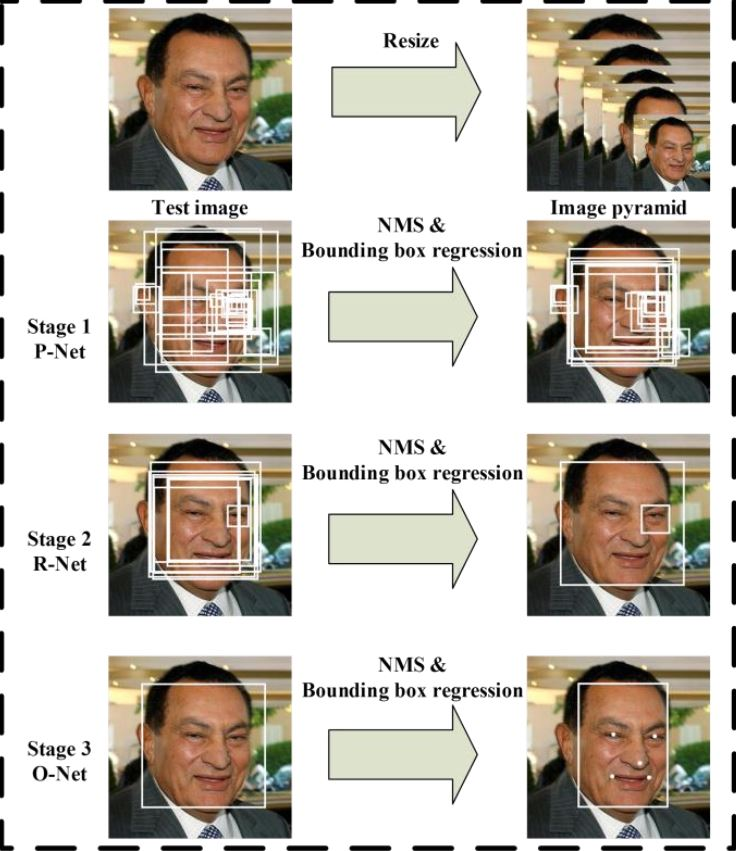
\includegraphics[height=7cm]{chap2/7.jpg}
	\bicaption{MtCNN 总体架构图\cite{zhang2016joint}}{MtCNN overall pipeline\cite{zhang2016joint}}
	\label{fig:mtcnn}
\end{figure}

在接收到一张图片之后,首先将其缩放得到图片金字塔。所得到的图像金字塔是三个级联卷积网络的输入。

第一阶段,我们使用一种全卷积网络叫做Proposal Network(P-Net)来获得候选人脸区域和它们的边界框回归向量。接着使用边界框回归向量去校准候选区域。最后使用非极大值抑制(NMS)整合高度重合的区域。

第二阶段,我们使用另一种卷积网络叫做Refine Network(R-Net)来进一步筛选得到的区域。在筛选结束之后,与第一阶段相同,使用边界框回归对人脸边界进行进一步校准。最后使用NMS整合重合区域。

第三阶段与第二阶段基本相似,但是在这一阶段我们主要对脸部更精细的特征进行描述。这一阶段使用Output Network(O-Net)得到人脸区域的五个特征点。

\subsection{Loss函数设计}

对于每一个样本$x_i$,人脸区域区分部分的Loss函数 其中$p_i$是网络输出结果是人脸区域的概率,$y_i^{det}\in\{0,1\}$是该区域是否是人脸的标签\cite{zhang2016joint}。
\begin{equation}
	L_{i}^{det}=-((y_{i}^{det}log(p_{i}))+(1-y_{i}^{det})(1-log(p_i)))
\end{equation}



边界框回归的Loss函数 其中$\hat{y}_i^{box}$是由网络得出的结果,$y_i^{box}$是实际的边界框\cite{zhang2016joint}。
\begin{equation}
	L_{i}^{box}=||{\hat{y}_i^{box}-y_i^{box}}||_2^2
\end{equation}



脸部特征回归的Loss函数与边界框类似,使用了Euclidean Loss\cite{zhang2016joint}。
\begin{equation}
L_{i}^{landmark}=||{\hat{y}_i^{landmark}-y_i^{landmark}}||_2^2
\end{equation}



\subsection{在CFDDB上的测试结果}

我们使用预训练完成的MtCNN在CFDDB上进行测试,测试中使用了TensorFlow 1.7.1 版本,并使用GPU加速网络运算。测试结果如表\ref{tab:mtcnn}所示,其中confidence表示所取MtCNN输出的人脸区域信任率,averageTime表示平均处理一张图片所需要的时间。

\begin{table}[!hpb]
	\centering
	\bicaption[MtCNN在CFDDB上的测试结果]
	{MtCNN在CFDDB上的测试结果}
	{MtCNN test results on CFDDB}
	\label{tab:mtcnn}
	\begin{tabular}{ cccc | c }
		\hline
		confidence & faceDetected & faceRight & averageTime & recall\\
		\hline
		0.90 & 433 & 388 & 344.38ms & $35.69\%$\\
		0.80 & 465 & 410 & 325.71ms & $37.71\%$\\
		0.70 & 483 & 423 & 357.41ms & $38.91\%$\\
		0.60 & 483 & 423 & 333.66ms & $38.91\%$\\
		\hline
	\end{tabular}
\end{table}

\subsection{结果分析}

\subsubsection{处理速度}

不同的confidence参数处理时间基本一致,均为350ms左右的时间处理一张宽1600像素,高1200像素的图片。由于使用了GPU加速运算,并且将原有的Matlab平台的代码成功移植到了更先进的TensorFlow平台,使得MtCNN处理速度符合我们的要求。

\subsubsection{准确率}

在CFDDB测试集中,MtCNN最多正确检测出了423个人脸区域,检测率最高为$38.91\%$,识别率较低,无法符合我们的要求。但是在WIDER FACE中的Hard测试集上,MtCNN都有着超过$60\%$的召回率\cite{zhang2016joint},然而在CFDDB上却无法体现。经过分析,可能的原因有以下两条:

\begin{figure}[!htp]
	\centering
	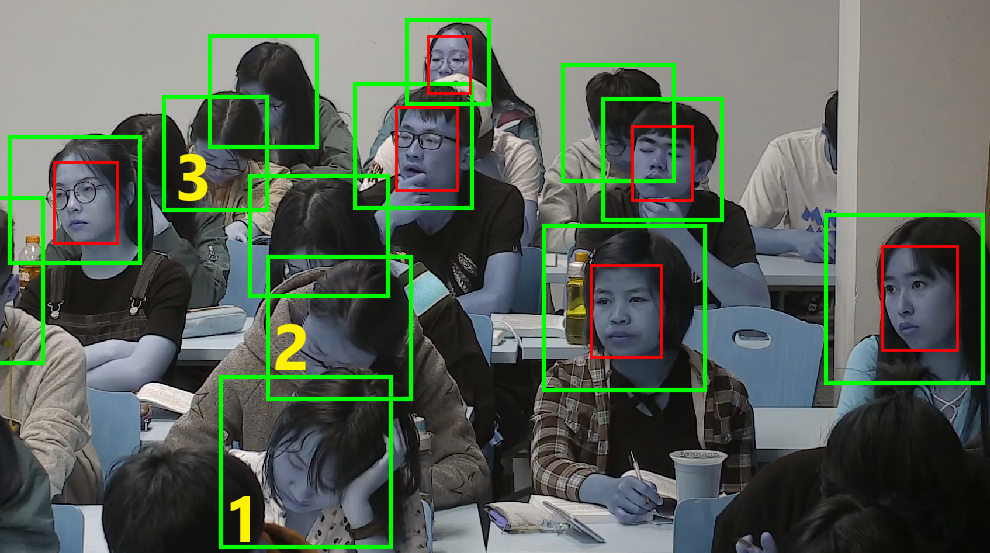
\includegraphics[height=5cm]{chap2/8.png}
	\bicaption{MtCNN 识别结果可视化样例}{MtCNN detect results example}
	\label{fig:mtcnn:accr}
\end{figure}


原因一:对侧脸的识别,五个特征点不完整的人脸识别率较低。CFDDB中有大量侧脸和不完整人脸,如图\ref{fig:mtcnn:accr}所示,其中人脸1俯仰左右都有较大的角度,难以识别;人脸2部分被遮挡,无法提取完整的五个特征点,因此被舍弃;人脸3俯仰角度过大,难以识别。


原因二:CFDDB数据分布的问题,由于数据中样本采集采用的从连续的视频中截取帧的方法,前后两次截取得到的图片差距不大,这样容易导致前一张图片中识别不出的图像往往在下一张图像中一样难以识别。这个问题需要通过扩充CFDDB的样本规模,去除相似度高的图像来解决。

\section{SSH检测器}

\subsection{概述}
SSH的全称为Single Stage Headless face detector\cite{najibi2017ssh},由Mahyar等人提出。SSH检测器针对小脸进行了优化,对处于自然环境的人脸识别有着非常好的效果。在WIDER FACE Hard测试集的测试中,SSH检测器的召回率达到了0.844,从检测效果来看,更加符合我们这个系统的需求。

与其他同样基于CNN的人脸检测器相比SSH检测器有如下四个特点:

首先,大多数基于CNN的人脸检测器只针对一种特定大小的人脸进行了训练。因此,在使用的时候需要先建立图像金字塔,然后对图像金字塔中的每一张图片在训练好的网络中前向传播,合并所有前向传播的输出得到结果。而SSH检测器设计了针对三种不同大小人脸的检测器,从不同的网络层中提取信息,使得SSH检测器在使用的时候只需要一次前向传播就可以完成所有大小的人脸检测而无需建立图像金字塔。

其次,大多数基于CNN的人脸检测器将人脸分为两个阶段。第一阶段,浅层的卷积特征图产生候选边界框集合。第二阶段,剩余的分类网络用于从集合中提取局部特征并将其分类。在这样的设计中,在第二阶段必须对第一阶段所有产生的候选框进行计算,从而需要极高的计算代价。而SSH检测器在一个阶段同时完成了边界框回归和最后的分类运算,因此计算代价更小。

再次,在达到国际领先的检测水平的同时,SSH检测器舍弃了基础VGG-16网络\cite{simonyan2014very}中含有大量参数的全连接层,使得训练过程更加容易。同时,也使得网络整体变得轻量快速。

最后, SSH检测器针对每个检测模块分别采用了Online hard negative and positive mining\cite{shrivastava2016training}的方法进行训练,使得训练得到的模型误报率更低,更加精确。

\subsection{网络结构}

图\ref{fig:ssh:arc}\cite{najibi2017ssh}展示了SSH检测器的总体架构。从图中可以看出,SSH检测器是一个全卷积深度网络,通过在步长分别为8、16和32的特征图上添加图\ref{fig:ssh:det}\cite{najibi2017ssh}所示的检测模块,实现了利用网络定位和区分人脸区域的功能。检测模块则由二元卷积分类器和回归运算模块组成。

\begin{figure}[!htp]
	\centering
	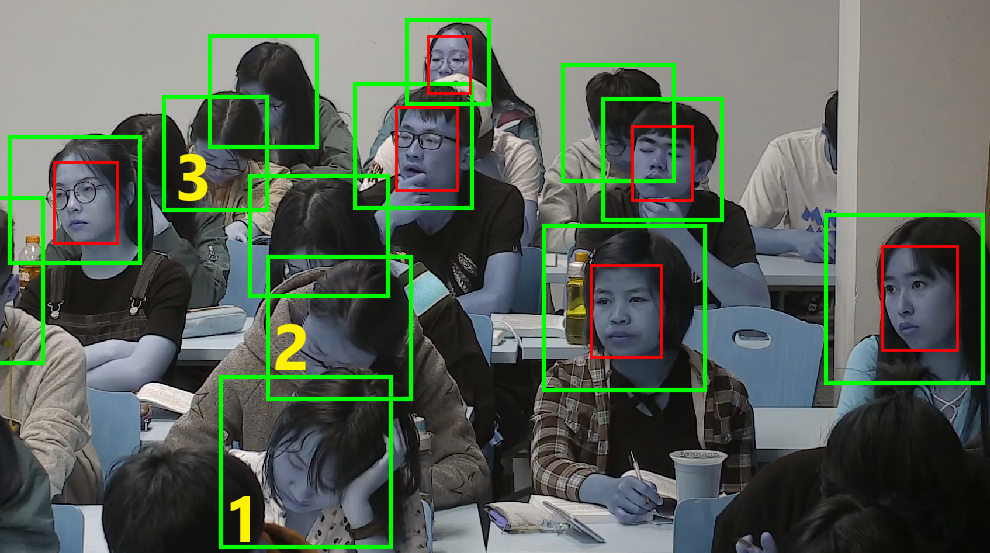
\includegraphics[height=7cm]{chap2/8.jpg}
	\bicaption{SSH 检测器总体架构\cite{najibi2017ssh}}{SSH face detector general architecture\cite{najibi2017ssh}}
	\label{fig:ssh:arc}
\end{figure}

\begin{figure}[!htp]
	\centering
	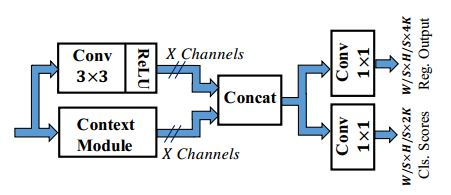
\includegraphics[height=3cm]{chap2/9.jpg}
	\bicaption{SSH 检测模块\cite{najibi2017ssh}}{SSH detection module\cite{najibi2017ssh}}
	\label{fig:ssh:det}
\end{figure}

\begin{figure}[!htp]
	\centering
	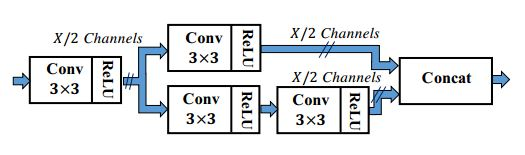
\includegraphics[height=3cm]{chap2/10.jpg}
	\bicaption{SSH 背景环境模块\cite{najibi2017ssh}}{SSH context module\cite{najibi2017ssh}}
	\label{fig:ssh:context}
\end{figure}

SSH检测器为单阶段检测器,并没有产生边界框候选集的阶段。事实上,SSH检测器通过对预先定义的边界框集进行回归而得到人脸区域的。而边界框集是通过密集的、重叠的滑动窗口所定义的。

而对于检测模块而言,有一系列的卷积层用于检测人脸的面部特征和位置定位,其中就包括了一个背景环境模块,如图\ref{fig:ssh:context}\cite{najibi2017ssh}。这个背景环境模块用于提高感受野的有效性,从而提高网络的检测精度。背景环境在人脸较小或者不清晰的时候可以向检测器提供非常重要的信息。因为当人脸面部信息被遮挡或者不清晰的时候,人脸周围的背景环境例如衣领、头发等信息可以作为面部区域的关键的辅助信息传入网络中,帮助网络断定这个区域是否为人脸区域。

事实上,在另一个由Peiyun Hu等人提出的Tiny face检测器\cite{hu2017finding}在论文中详细叙述了背景区域对于小脸检测的重要性。根据论文中的叙述,增加背景环境信息几乎总是有效的,无论对于大脸还是小脸。Peiyun Hu等人在实验中发现唯一降低了识别准确率的情况是向宽25像素,高25像素的小脸区域加入了超过宽300像素,高300像素的背景信息区域。而这种情况识别率降低的主要原因是向感受野中加入了明显过多的背景信息而导致了检测器出现了过拟合现象。


\subsection{在CFDDB上的测试结果}
\label{chap2:sshresult}

我们使用预训练完成的SSH检测器在CFDDB上进行测试,选用Caffe作为框架平台,测试中使用了GPU加速网络运算。测试结果如表\ref{tab:ssh}所示,其中confidence表示所取SSH检测器输出的人脸区域信任率,averageTime表示平均处理一张图片所需要的时间。

\begin{table}[!hpb]
	\centering
	\bicaption[SSH检测器在CFDDB上的测试结果]
	{SSH在CFDDB上的测试结果}
	{SSH test results on CFDDB}
	\label{tab:ssh}
	\begin{tabular}{ cccc | c }
		\hline
		confidence & faceDetected & faceRight & averageTime & recall\\
		\hline
		0.90 & 921 & 854 & 235.93ms & $78.56\%$\\
		0.80 & 957 & 885 & 235.41ms & $81.42\%$\\
		0.70 & 975 & 900 & 236.19ms & $82.80\%$\\
		0.60 & 989 & 913 & 224.73ms & $83.99\%$\\
		0.50 & 1008 & 929 & 227.33ms & $85.46\%$\\
		\hline
	\end{tabular}
\end{table}

\subsection{结果分析}

\subsubsection{处理速度}

不同的confidence参数处理时间基本一致,均为230ms左右的时间处理一张宽1600像素,高1200像素的图片。由于使用了GPU加速运算,而且SSH检测器使用了轻量的网络,使得处理时间完全满足系统需求。

\subsubsection{准确率}

在CFDDB测试集中,SSH检测器最多正确检测出了998个人脸区域,识别率高达$91.81\%$。即使将confidence参数调高至0.9,识别率任然达到了$85.1\%$,超过了$80\%$的要求。因此,SSH检测器的准确率完全可以满足系统的需求,适合作为人脸检测模块的核心算法。

\subsection{网络优化与平台移植}

虽然SSH检测满足了我们的检测条件,但是我们在测试中也发现了SSH存在的一些待改进的问题。

首先,SSH检测器目前只有Caffe平台的实现,这对于测试和部署都是一项极大的挑战。Caffe平台虽然功能强大,但是搭建GPU支持的Caffe环境却必须从源码进行编译。这就意味和每次部署搭建环境时都必须安装数量庞大的依赖库,并下载源码编译。整个过程需要耗费大量的时间,不利于规模性部署。而且随着Caffe平台的维护力度逐渐减小,最新版本的显卡驱动和深度神经网络加速库均无法使用,使得网络的运行效率下降。同时,Caffe平台对于嵌入式设备的支持优化较少,不利于将识别模块移植到嵌入式平台上使用。

其次,SSH检测器基于性能较弱的VGG-16网络\cite{simonyan2014very}改进而来,存在提升的空间。如果将其中的VGG-16网络替换为对应的MobileNets网络\cite{howard2017mobilenets},或者MobileNetsV2网络\cite{sandler2018inverted},则不仅可以提升网络的运行速度,而且更方便将网络移植到嵌入式设备等没有GPU支持的设备中使用。

最后,SSH检测器难以兼容使用TensorFlow平台实现的人脸识别算法。由于Caffe平台和TensorFlow平台使用了不同版本的Protocol Buffer依赖库,如果希望能够同时运行两个平台就需要安装老旧版本的TensorFlow平台并进行一些繁琐的设置。这不仅损失了人脸识别算法的运行效率,而且给规模化部署带来了更多的挑战。

\section{Tiny face检测器}

\subsection{概述}

Tiny face检测器\cite{hu2017finding},是由Peiyun Hu等人提出的一种针对小脸进行优化处理的人脸检测器,也是最早针对小脸进行检测的深度网络之一。Tiny face使用了图像金字塔和多种不同大小、不同宽高比的模板来检测不同大小人脸,并基于VGG-16网络\cite{simonyan2014very},ResNet-101和ResNet-50网络\cite{he2016deep}结构都进行了实现。其中基于ResNet-101的实现在WIDER FACE测试集Hard部分的召回率达到了0.823\cite{hu2017finding}。

\subsection{在CFDDB上的测试结果}
\label{chap2:tinyresult}

我们使用在TensorFlow平台上预训练完成的Tiny face检测器在CFDDB上进行测试,测试中使用了GPU加速网络运算。测试结果如表\ref{tab:ssh}所示,其中confidence表示所取Tiny face检测器输出的人脸区域信任率,averageTime表示平均处理一张图片所需要的时间。

\begin{table}[!hpb]
	\centering
	\bicaption[Tiny face检测器在CFDDB上的测试结果]
	{Tiny face检测器在CFDDB上的测试结果}
	{Tiny face detector test results on CFDDB}
	\label{tab:tiny}
	\begin{tabular}{ cccc | c }
		\hline
		confidence & faceDetected & faceRight & averageTime & recall\\
		\hline
		0.90 & 1068 & 953 & 1906.05ms & $87.67\%$\\
		0.80 & 1070 & 953 & 1792.24ms & $87.67\%$\\
		0.70 & 1074 & 952 & 1859.22ms & $87.58\%$\\
		0.60 & 1077 & 958 & 1888.82ms & $88.13\%$\\
		0.50 & 1082 & 961 & 1801.81ms & $88.41\%$\\
		\hline
	\end{tabular}
\end{table}

\subsection{结果分析}

\subsubsection{处理速度}

不同的confidence参数处理时间基本一致,均为1850ms左右的时间处理一张宽1600像素,高1200像素的图片。时间大约为SSH检测器处理时间的8~9倍,而且远超大于系统所要求的500ms时间,不符合系统的要求。

\subsubsection{准确率}

在CFDDB测试集中,Tiny face检测器最多正确检测出了1082个人脸区域,识别率高达$88.41\%$。即使将confidence参数调高至0.9,识别率任然达到了$87.67\%$,超过了$80\%$的要求。因此,Tiny face检测器的准确率满足系统的需求。

\subsubsection{与SSH检测器的对比分析}

从表\ref{tab:ssh}和表\ref{tab:tiny}可以看出,在运算效率上,SSH检测器优势非常大。原因主要是SSH能够一次性检测多种大小的人脸而不依赖于图像金字塔,避免了在多个尺度处理同一张图片的运算,从而获得了更高的运算效率。

如果不考虑运算效率,而希望得到召回率高而误判率低的算法,则需要计算两种算法在CFDDB上的参数$\alpha$得到表\ref{tab:tinyandssh}所示的结果:

\begin{table}[!hpb]
	\centering
	\bicaption[Tiny face检测器与SSH检测器对比分析表]
	{Tiny face检测器与SSH检测器对比分析表}
	{Tiny face detector and SSH detector comparision table}
	\label{tab:tinyandssh}
	\begin{tabular}{ c|ccc|ccc }
		\hline
		confidence & recall(Tiny) & errorrate(Tiny) &$\alpha$(Tiny) & recall(SSH)& errorrate(SSH)& $\alpha$(SSH)\\
		\hline
		0.90  & $87.67\%$& $10.58\%$& 2.1986 & $78.56\%$& $6.16\%$& 1.8892\\
		0.80  & $87.67\%$& $10.76\%$& 2.2170 & $81.42\%$& $6.62\%$& 1.8906\\
		0.70  & $87.58\%$& $11.22\%$& 2.2642 & $82.80\%$& $6.90\%$& 1.8978\\
		0.60  & $88.13\%$& $10.95\%$& 2.2294 & $83.99\%$& $6.99\%$& 1.8898\\
		0.50  & $88.41\%$& $11.13\%$& 2.2443 & $85.46\%$& $7.27\%$& 1.8968\\
		\hline
	\end{tabular}
\end{table}

根据$\alpha$的定义知,当召回率越高的时候$\alpha$的值越小,当误判率越低时$\alpha$的值越小,因此,$\alpha$的值越小,代表了当前检测算法的性能越优秀。从表\ref{tab:tinyandssh}中可以清晰的看出,无论参数confidence的值是多少,SSH检测器的$\alpha$值总是小于Tiny face检测器的$\alpha$值。因此,综合考虑召回率和误判率的情况下,SSH检测器依然优于Tiny face检测器。





%\chapter{人脸识别算法}
\label{facerecognition}

在检测到人脸区域的之后就需要对区域内的人脸图像进行特征提取和识别。目前最先进的人脸识别思路是将人脸 图片经过深度神经网络的处理得到高维的人脸特征向量。然后使用这些特征向量进行人脸搜索、人脸分类和人脸识别。

事实上,我们可以将得到高维人脸特征向量的过程看作是一种映射。我们使用的深度神经网络就是一种映射函数。相同或相似的人脸图像由这种映射函数得到的向量具有较近的距离,而差异较大的人脸图像经过映射得到的向量具有较远的距离。

特征向量间的距离定义也有很多种,有些是欧式距离,有些是角度距离。而如果网络输出的特征向量都进行了标准化处理,就可以用两个特征向量的点积作为距离的衡量标准。在这种情况下,两个特征向量的点积越接近1,则两个特征向量对应的人脸就越相像;越接近-1,则两个特征向量对应的人脸差异越大。

在实际算法中,大多数算法在识别之前都有将人脸校正的需要。校正操作就是通过检测到人脸的多个特征点进行运算,从而将带有较大角度的人脸转换为相应正脸的过程。由于这种过程需要检测人脸的特征点,大多数算法都使用了在人脸检测算法中提到的MtCNN网络进行校正操作。

如果全部可识别的人脸数量为$face_{all}$,识别正确的人脸数量为$face_{right}$定义召回率$recall$为:

\begin{displaymath}
\label{eq:rrdef}
recall = \frac{face_{right}}{face_{all}} 
\end{displaymath}

由于CFDDB目前只能粗略测得人脸识别算法的准确性,我们要求合格的人脸识别算法需要$recall>50\%$。

\section{ArcFace简介}

使用深度神经网络检测人脸的方法有很多,它们主要的不同点有三个:

第一,训练数据。对于深度神经网络而言,通常训练数据越多,得到的模型就越精确。人脸识别中使用的公开训练数据集主要有VGG-Face[19],VGG2-Face[20],CAISA-WebFace[21],UMDFaces[22],MS-Celeb-1M[23]和Megaface[24]。而Google等公司的私有数据集甚至拥有数百万的不同人脸数据,可以训练出商用的人脸识别网络。

第二,网络结构。与使用CNN网络的人脸检测器类似,研究者们也为人脸识别设计了许多不同的网络。常见的有ResNet系列网络[25],VGG系列网络[26]和MobileNets等等。

第三,Loss函数。不同的神经网络有着不同的Loss函数设计,常见的有Euclidean margin based loss和Angular and cosine margin based loss两大类。

而ArcFace[28]所使用的训练数据为MS-Celeb-1M[23]数据集,网络结构基于VGG2[27],使用一种全新提出的additive angular margin作为Loss函数。

\section{在CFDDB上的测试结果}

下表\ref{tab:arcface}展示了ArcFace在CFDDB上的测试结果。其中参数confidence表示两特征向量的最小信任值。即如果一张图片的特征向量与人脸标准数据库中所有的特征向量的点积值均低于confidence,则认为该图片中的人脸不属于人脸标准数据库中的任何一张人脸。参数faceRecongnized参数表示当前属于人脸标准数据库中的人脸数量,参数faceRecognizeRight表示识别正确的人脸数量。

\begin{table}[!hpb]
	\centering
	\bicaption[ArcFace在CFDDB上的测试结果]
	{ArcFace在CFDDB上的测试结果}
	{ArcFace test results on CFDDB}
	\label{tab:arcface}
	\begin{tabular}{ ccc | c }
		\hline
		confidence & faceRecognized & faceRecognizeRight &  recall\\
		\hline
		0.90 & 249 & 193 & $77.51\%$\\
		0.80 & 412 & 558 & $73.84\%$\\
		0.70 & 543 & 711 & $76.37\%$\\
		0.60 & 838 & 649 & $77.44\%$\\
		0.50 & 916 & 691 & $75.44\%$\\
		\hline
	\end{tabular}
\end{table}

分析表\ref{tab:arcface}中的测试结果可以看出,调整confidence参数从0.5至0.9,召回率均超过$70\%$,符合系统的要求。
\chapter{人脸匹配算法}

\section{概论}

由人脸识别模块得到人脸特征向量之后,接下来就需要将这个特征向量与人脸标准数据库中已有的特征向量进行匹配,找到距离其最近的特征向量,从而确定待检测人脸的身份。如果数据库中的数据量较少,采用线性搜索的性能就足以满足系统需求。但在数据量较大,例如百万以上的特征向量时,线性搜索需要较多的时间,无法满足我们系统实时性的需求。因此,我们需要更高效的搜索算法加速这一过程。

我们对合格的人脸匹配算法有四点要求:

第一是准确,一次查询的结果应当非常接近线性搜索的结果。第二是快速,算法的时间复杂度为$O(1)$或者$O(\log{}N)$。第三是高效,即理想情况下,数据的索引应当和数据集成线性关系。第四是高维,由于人脸特征向量的维度均在100维以上,算法需要支持对高维特征的高效搜索。

除了线性搜索,常见的精确搜索算法有基于树形结构的R-tree和K-D tree等算法,根据论文[1]的研究结论,在维度超过10的时候,这些精确算法的时间效率已经超过了线性搜索,而人脸特征向量的维度基本上在100的级别。所以使用这些精确搜索算法无法满足高维的要求,这些算法都不合适用作本系统的匹配算法。

而在机器学习的领域,支持向量机(SVM)常用于高维向量的分类和回归。而在人脸向量的匹配阶段,如果人脸特征数据库内存在n个特征向量, 那么我们使用SVM将找到查询向量$\mathbf{q}$所匹配的特征向量共有两种思路:

思路一,训练$n$个分类器,每个分类器都将人脸特征库中的某一个特征向量与剩余的所有特征向量区分开。在使用时,需要每个分类器对查询向量$\mathbf{q}$进行分类,如果$\mathbf{q}$与某个特征向量分到了同一类,则将该特征向量作为$\mathbf{q}$的匹配候选项。

思路二,训练$C_n^2$个分类器,将$n$个特征向量中任意挑出的一对不同的特征向量区分开。需要找到查询向量$\mathbf{q}$的匹配项时,使用每个训练好的分类器对$\mathbf{q}$进行分类,每次将分类器输出结果所表示的特征向量类别权重加一。所有的分类器分类完毕时,选择权重最高的一类中的特征向量即为匹配结果。

这两种思路在n不大的时候都是可行的。事实上,在一些简单的人脸识别系统中,使用多类支持向量机 (Multi-Class SVM)匹配高维人脸特征向量的做法非常普遍。

然而对于思路一中的方法,当n非常大的时候,需要训练的分类器的数量为$O(n)$,而且每次查询的时间复杂度也为$O(n)$;对于思路二中的方法,当n非常大的时候,需要训练的分类器的数量为$O(n^2)$,每次查询的时间复杂度也为$O(n^2)$。在简单分析后我们可以看出,多类支持向量机不符合快速的要求,当人脸特征向量的数量非常大的时候,不适合作为人脸匹配算法使用。

我们注意到人脸特征向量的具有这样的特性:相同身份的人脸会产生距离较近的特征向量,而不同身份的人脸往往会产生距离较远的特征向量。由此可将人脸特征向量的匹配过程等同于在人脸特征向量数据库中寻找距离查询向量$\mathbf{q}$距离最近的一项。通过这样的转换,我们将匹配问题等价于最近邻搜索问题。

最近邻搜索问题的解决主要有两大类方法,精确搜索和近似搜索。其中近似搜索是一类能够以非常高的概率找到最近邻的搜索方法。

\section{基于局部敏感哈希的近似搜索}

\subsection{LSH函数族的定义与生成}

局部敏感哈希(LSH)在最近邻的搜索问题上有着广泛的应用,是一种近似搜索方法。

LSH算法的核心是LSH函数族,以下为LSH函数族的定义[1]:

一个LSH函数族$\mathcal{F}$定义在矩阵空间$\mathcal{M}=(M,d)$上,其中阈值$R>0$,渐进系数$c>1$。LSH函数族中的每一个函数$h:\mathcal{M}\rightarrow S$都将元素从矩阵空间映射到桶$s\in S$中,并满足使用随机平均抽取的一个函数$h\in \mathcal{F}$,为对任意的两个点$p,q\in \mathcal{M}$,都有如下特性:

\begin{itemize}
	\item 若$d(p,q)\leq R$,那么$h(p)=h(q)$的概率至少为$P_1$。
	\item 若$d(p,q)\geq cR$,那么$h(p)=h(q)$的概率至多为$P_2$。
\end{itemize}

在最邻近搜索中使用的LSH函数族均满足$P_1>P_2$的条件,此时,这个LSH函数族被称为$(R,cR,P_1,P_2)-sensitive$。

如果给定一个$(d_1,d_2,p_1,p_2)-sensitive$的LSH函数族$\mathcal{F}$,我们可以通过与或的操作创建新的LSH函数族。

采用求与的方法,定义一个新的函数族$\mathcal{G}$,函数族中每一个哈希函数为$g$。每一个$g$均由函数族$\mathcal{F}$中的$k$个随机选取的哈希函数$h_1,...,h_k$构成。对于哈希函数$g\in \mathcal{G}$,$g(x)=g(y)$当且仅当$i=1,2,...,k$时,所有的$h_i(x)=h_i(y)$。此时生成$\mathcal{G}$为$(d_1,d_2,p_1^k,p_2^k)-sensitive$的LSH函数族。

采用求或的方法,定义一个新的函数族$\mathcal{G}$,函数族中每一个哈希函数为$g$。每一个$g$均由函数族$\mathcal{F}$中的$k$个随机选取的哈希函数$h_1,...,h_k$构成。对于哈希函数$g\in \mathcal{G}$,$g(x)=g(y)$当且仅当存在一个或者多个$i$,使得$h_i(x)=h_i(y)$。此时生成$\mathcal{G}$为$(d_1,d_2,1-(1-p_1^k),1-(1-p_2^k))-sensitive$的LSH函数族。

\subsection{基础LSH最邻近搜索算法}

利用LSH函数族进行最近邻搜索的算法有两个主要参数,宽度$k$和哈希表的数量$L$,其中宽度$k$由创建过程中随机选取哈希函数的数量$k$定义。

第一步,采用上述的求与或求或的方法创建新的LSH函数族$\mathcal{G}$,接着由LSH函数族$\mathcal{G}$中随机选区$L$个不同的哈希函数,创建$L$个哈希表。

第二步,对于查询向量$\mathbf{q}$,遍历每一个哈希表,取出与其分配到同一桶中的的向量将其放到集合$S$中。

第三步,使用线性搜索的方法找到$S$中最邻近$\mathbf{q}$的向量。

\subsection{基础LSH最邻近搜索算法复杂度分析}
令
\[k=\frac{log n}{log 1/P_2},L=n^\rho\]

其中
\[\rho =\frac{log P_1}{log P_2}\]

则该算法的空间复杂度为$O(n^{1+\rho})$,时间复杂度为$O(n^\rho)$。由于$0<\rho <1$,所以该算法的搜索的时间效率高于线性搜索。

从工程实践的角度出发,基础LSH算法的最大问题是需要非常多的哈希表,从而在保证准确性的同时找到绝大多数的临近元素。而每个哈希表的空间大小是和数据集的大小成比例的,所以数据量越大,需要的存储空间就越大。如果哈希表的存储空间超过了内存的容量,那么每一次查询操作就会涉及到磁盘的读取,从而极大的增加每次查询操作的时间开销。

\subsection{基础LSH最邻近算法的优化思路}

优化基础LSH最邻近算法的一种思路是减少查询时所需要的哈希表的数量。假设我们知道待求的最邻近向量$\mathbf{p}$和查询向量$\mathbf{q}$之间的距离$R_p$,那么原则上来说,我们可以计算出$\mathbf{p}$与$\mathbf{q}$在同一个桶里面的概率。如果定义这个概率叫做成功率,那么查询的时候只需要查找成功率高的桶就可以避免使用过多无用的哈希表,从而提高存储的利用率。

然而预先计算每个桶的成功率在实际情况下是十分复杂的,所以,我们需要一种方法来高效的进行这种计算。每次查询之前,随机生成一个与查询向量$\mathbf{q}$相距$R_p$的点$\mathbf{p'}$。标记$\mathbf{p'}$进过哈希后落到的桶。这样保证了所有的桶取样概率的正确性。多次执行同样的操作,即可找出所有高成功率的桶。

这样的思路以牺牲时间效率为代价换取了更高的空间利用率,避免了内存不够而需要访问硬盘的情况。根据论文[3]的实验结果,这样的优化方式使得需要的哈希表数量减少了$1/2$到$2/3$。不过由于每次查询前都增加了取样的过程,使得每次查询的时间增加了$30\%$到$210\%$不等。

除了每次查询需要更多的时间之外,在实际测试中还发现了上述思路存在其他一些缺陷。

第一,在一次查询中高成功率的桶会被不同的扰动点$\mathbf{p'}$产生多次,即在一次查询中做了多次重复计算。通过记住每个扰动点生成的桶可以避免此问题,而其需要的空间开销在高并发量的查询时仍然是不可接受的。

第二,对于每一个待检测的数据集,参数$R_p$需要人工调整。若$R_p$偏大,则取样结果过多,容易产生误判;若$R_p$偏小,则取样结果过少,容易产生缺漏。

针对上述的缺陷,Qin Lv等人在论文[3]中提出了多探针LSH,以在减少哈希表数量的同时可以高效的执行查询操作。

设$\mathbf{a}$为从正态分布中随机取出的$d$为向量,$b$是从$[0,W]$均匀分布中随机取出的一个实数,则LSH函数族中的每一个哈希函数被定义为:
\[
h_{\mathbf{a},b}(\mathbf{v})=\Big\lfloor\frac{\mathbf{a}\cdot \mathbf{v}+b}{W} \Big\rfloor
\]

根据这个哈希函数的性质,如果$\mathbf{p}$,$\mathbf{q}$两点为邻近点,而经过哈希函数的计算后$\mathbf{p}$没有和$\mathbf{q}$分在同一个桶中,那么$\mathbf{p}$一定与$\mathbf{q}$分到了靠近的桶中。事实上,如果参数$W$选取合适,$\mathbf{p}$会有极大的概率分到与$\mathbf{q}$紧邻的桶中。

根据邻近点在桶中的分布特性,使用合适的方法推导出探针序列,即可使用探针将绝大多数查询向量$\mathbf{q}$的邻近点找出,从而得到最邻近点。

在论文[3]中,使用了两个数据集来测试多探针LSH算法,一个是包含130万图片的数据集,另一个是含有260万音频的数据集。测试结果表明,多探针LSH算法的空间利用率是基础LSH算法的14至18倍,而查询时间基本接近。


\section{基于邻近图的近似搜索}

\subsection{概述}

基于LSH进行近似搜索的算法主要思想是相似的向量经过哈希函数的计算后仍然在相邻或者相同的桶里。这类算法在数据集中的高维向量距离相距较远的情况下存在明显的缺陷,即相邻的样本在计算会分布在稀疏的、不相邻的桶中,从而降低搜索效率。相比于LSH,使用有向图来描述数据集则可以很好的解决这个问题。数据集中的每个特征向量都由有向图中的一个顶点表示。Ben Harwood与Tom Drummond在论文[4]中提出了一个高效的利用邻近图执行近似搜索的算法。

\subsection{理想图的构建}

如何构建邻近图是这类算法的核心。而最优的邻近图是在理想图的基础上优化而来。因此,在得到邻近图之前首先需要构建一个理想图。当查询点$Q$为数据集中的一个点时,无论初始查询下标从哪里开始,算法\ref{algo:fanng1}总能正确的找到正确的匹配结果。符合这样要求的最小图定义为理想图。

\begin{algorithm}
	% \begin{algorithm}[H] % 强制定位
	\caption{向下搜索算法}
	\label{algo:fanng1}
	\begin{algorithmic}[1] %每行显示行号
		\Require $P$理想图的顶点集,$E$理想图的边集,$Q$查询点,$v$初始查询下标 % 输入
		\Ensure $v$最邻近下标 % 输出
		\For {each edge $E_i$ with start vertex $P_v$}
		\State $u\leftarrow$ index of end vertex of $E_i$
		\If {$distance(Q,P_u)<distance(Q,P_v)$}
		\State $v\leftarrow u$
		\EndIf
		\EndFor
	\end{algorithmic}
\end{algorithm}

在这样的搜索过程中,每次迭代后当前的点与查询点之技安的距离都会减小。因此,整个算法在有限次迭代之后一定会终止。这也同时意味着如果图中存在一条从$p_1$到$p_2$的边,那么任何一条从$p_1$出发到$p_3$的边,当$p_1$到$p_3$的距离比$p_2$到$p_3$的距离远时都没有存在的意义。

在理想图中,如果给定数据点$p_i$与距离函数$d:\mathbf{R}\times \mathbf{R} \rightarrow \mathbf{R}$,定义边$(p_1,p_2)$阻塞边$(p_1,p_3)$当且仅当$d(p_1,p_2)<d(p_1,p_3)$并且$d(p_2,p_3)<d(p_1,p_3)$。

明确了如何精简图之后,使用算法\ref{algo:fanng2}构建理想图。

\begin{algorithm}
	% \begin{algorithm}[H] % 强制定位
	\caption{理想图构建算法}
	\label{algo:fanng2}
	\begin{algorithmic}[1] %每行显示行号
		\Require $P$理想图的顶点集
		\Ensure $E$理想图的边集 % 输出
		\For {each vertex $P_i$}
		\State $e\leftarrow$ empty sorted list of edges
		\For {each vertex $P_j\neq P_i$}
		\State $u \leftarrow$ index of end vertex of $e_j$
		\State $L \leftarrow$ length of $e_j$
		\State $occluded \leftarrow \mathbf{false}$
		\For {each edge $E_k$ with start vertex $P_i$}
		\State $v \leftarrow$ index of end vertex of $E_k$
		\If {$d(P_u,P_v)<L$}
		\State $occluded \leftarrow \mathbf{true}$
		\EndIf
		\EndFor
		\EndFor
		\EndFor
		\Return $E$
	\end{algorithmic}
\end{algorithm}

建立理想图之后我们需要探究其存储空间是否合理。尽管数据集中的数据可能是高维的,例如SIFT[5]数据集中的数据有128维,但是其固有维度却只有11维。这使得使用SIFT数据集构建的理想图中每个点的度平均值为25左右。因此,图的存储空间是可以接受的。

不过此时,我们要求查询点$Q$必须在数据集中,这样的要求限制了算法的运用场景。所以,我们将阻塞的定义修改为:边$(p_1,p_2)$阻塞边$(p_1,p_3)$当且仅当$d(p_1,p_2)<d(p_1,p_3)$并且$d(p_2,p_3)^2<d(p_1,p_3)^2-2\tau d(p_1,p_2)$。此时再使用算法\ref{algo:fanng2}即可构建寻找与查询点$Q$距离小于$\tau$的最邻近点的理想图。

需要注意的是,如果使用了新的阻塞定义,会增加理想图中每个点的度,使得整个图的存储代价变大,同时也会使一次搜索的时间效率下降。因此,在实际使用时,需要根据需要权衡$\tau$的取值。如果$\tau$值选的过小,则很可能降低可能的最邻近点的候选数量;如果$\tau$值选的过大,则很可能增大存储图所需要的空间并降低搜索的时间效率。

\subsection{使用回溯进行快速搜索}

一个提高搜索效率的方法通过修改算法\ref{algo:fanng1}。新的算法\ref{algo:fanng3}不再像算法\ref{algo:fanng1}当无法继续时终止,而是使用了深度优先的回溯搜索来检查从第二靠近的点出发,依然没有被搜索过的边。如果第二近的点所有的边都被搜索过了,那么检查第三靠近的点,以此类推。具体实现的时候需要维护一个尚未搜索过边的优先级队列。搜索一条边包括了首先计算查询点到有向边的终点的距离,然后根据距离长短替换优先级队列中的边,短边优先。

这里需要权衡的一项参数时距离的计算次数,当计算次数达到一个上限$M$后,返回距离查询点最近的点。

\begin{algorithm}
	% \begin{algorithm}[H] % 强制定位
	\caption{快速搜索算法}
	\label{algo:fanng3}
	\begin{algorithmic}[1] %每行显示行号
		\Require $P$邻近图的顶点集,$E$邻近图的边集,$Q$查询点,$v$初始查询下标,$M$最大计算次数 % 输入
		\Ensure $n$最邻近下标 % 输出
		\State $X\leftarrow$ empty priority queue
		\State add edge $e_0$ with start vertex $P_v$ to $X$
		\State $m\leftarrow 1$
		\State $n\leftarrow v$
		\While {$m<M$}
		\State $e_i\leftarrow$ remove top of $X$
		\State $u\leftarrow$ index of end vertex of $e_i$
		\If {$P_u$ has not been searched yet}
		\State add edge $e_0$ with start vertex $P_u$ to $X$
		\State $m\leftarrow m+1$
		\If {$d(Q,P_u)<d(Q,P_n)$}
		\State $n\leftarrow u$
		\EndIf
		\EndIf
		\State $v\leftarrow$ index of start vertex of $e_i$
		\If {$i<$ number of edges with start vertex $P_v$}
		\State add edge $e_{i+1}$ with start vertex $P_v$ to $X$
		\EndIf
		\EndWhile
		\Return $n$
	\end{algorithmic}
\end{algorithm}

\subsection{邻近图的快速构建}

由于对$n$个中的每个点的$n$种距离进行了排序,算法\ref{algo:fanng2}构建图的时间复杂度为$O(n^2\log{n})$,这样的时间复杂度使得建立邻近图的时间代价非常高,因此我们需要一种更有效的思路来构建邻近图。

这种思路使用了同时使用了两种不同的方法。其中第一种方法首先从数据集中随机选取了两个点$v_1$和$v_2$,然后使用算法\ref{algo:fanng1}尝试从$v_1$出发搜索$v_2$。如果目前的图为空图,这种方法会直接在$v_1$和$v_2$之间添加一条边。如果不是空图,则需要检验新加入的边是否造成了边的阻塞,如果有阻塞发生,则将较长的边移除以消除阻塞。如果数据集的大小为$N$,重复这种操作直至$50N$次调用算法\ref{algo:fanng1}平均成功率超过$90\%$为止。

当算法\ref{algo:fanng1}被不断调用时,图的构建过程会渐渐减慢,此时使用第二种方法来进一步提升图的完整性。第二种方法调用搜索算法返回几千个点的近邻点以构建近邻列表。遍历这个近邻列表并调用算法\ref{algo:fanng2}去除阻塞边。并行对数据集中的每个点都应用这种方法可以快速高效的构建邻近图。

\subsection{复杂度}

根据论文[4]中的实验结果,基于邻近图的近似搜索算法的时间复杂度约为$O(N^{0.2})$,其中$N$为数据集中的数据量。因此,这种方法符合我们的系统准确、快速、高效、高维的要求。作者同时还提供了基于这个方法实现的开源工具包,极大的方便了系统的实现与使用。

\section{基于kNN图}



\chapter{系统架构设计}

\section{概述}

无感知人脸识别系统的架构设计主要分为三部分:数据处理流程、设备网络拓扑结构和系统逻辑架构。其中,数据处理流程主要描述系统中的数据存储结构,数据格式和数据流动情况。设备网络拓扑结构主要描述系统中所有机器的物理部署特征,网络拓扑等。系统逻辑架构主要描述系统实现代码中所有的模块和组件,以及不同模块组件之间的交互与职能分配。

\section{数据处理流程}

无感知人脸识别系统的数据处理流程如图\ref{fig:chap5:data}所示:

\begin{figure}[!htp]
	\centering
	\includegraphics[height=1.7cm]{chap5/1.jpg}
	\bicaption[系统数据处理流程图]
	{系统数据处理流程图}
	{System data architecture}
	\label{fig:chap5:data}
\end{figure}

图\ref{fig:chap5:data}中标注为1的部分表示视频流的帧截取过程;标注2的部分代表人脸区域检测的过程;标注3的部分代表人脸识别的过程;标注4的部分代表人脸匹配的过程。

最先进入系统的是由摄像设备和嵌入式设备获取的视频流数据,这部分数据在本地进行帧截取操作后会将获得的图片上传到图片队列中。图片队列是一个被服务器维护的优先级队列,其长度根据系统的需求和服务器的性能确定。每接收到一张新的图片时,首先检查队列是否已满。如果队列已满,则将该图片丢弃,并向用户发送服务器繁忙的信息。如果队列未满,则根据该图片的优先级将该图片插入到队列中。队列中的每张图片都应有唯一的标记,以表明这张图片的发送源。

进行人脸检测时,每次从图片队列的前端取出一张图片进行检测,检测完成后根据图片标记将得到的人脸区域做好标记插入到人脸队列中。如果人脸队列已满,则将带标记的人脸区域存储在服务器中的特定硬盘区域。当人脸队列有空余位置时,从该硬盘区域中读取存储的内容加入人脸队列的尾部,并删除硬盘中的相应内容。

进行人脸识别时,每次从人脸队列的前端取出批尺寸大小的人脸图像及其标记加载到人脸识别模块中,得到批尺寸大小的特征向量及标记。接着将这些特征向量及其标记发送到人脸数据库中进行匹配。由于不同的请求之间没有数据依赖性,匹配模块可以在高并发量的情况下运行,得到匹配的身份信息与每条信息的初始标记。

最后,根据每条身份信息的标记,将某一用户请求的所有身份信息返回给用户。

\section{设备网络拓扑结构}

无感知人脸识别系统的设备网络拓扑结构如图\ref{fig:chap5:phy}所示:

\begin{figure}[!htp]
	\centering
	\includegraphics[height=4cm]{chap5/2.jpg}
	\bicaption[系统设备网络拓扑结构图]
	{系统设备网络拓扑结构图}
	{System physical architecture}
	\label{fig:chap5:phy}
\end{figure}

图\ref{fig:chap5:phy}中的标注1的部分表示摄像设备与GPU服务器集群之间通过有线网络连接,数据从摄像设备传输到GPU服务器集群;标注2表示嵌入式设备与GPU服务器集群之间通过无线网络连接,数据从嵌入式设备传输到GPU服务器集群;标注3表示GPU服务器集群与人脸数据库之间通过内部的有线网络连接;标注4表示人脸数据库与交互服务器通过内部的有线网络连接。

其中,人脸检测模块和人脸识别模块部署在GPU服务器集群中,人脸匹配模块部署在人脸数据库中。交互服务器负责分析匹配结果,并将分析后的信息发送到相应的用户设备中。

在系统的实际部署中,由于摄像设备和嵌入式设备的输入众多,网络拓扑结构会更为复杂,网络中很可能需要增加一些中间节点。如果GPU服务器集群不在本地而在云端,则整个网络传输就无法在一个局域网内进行。此时则需要考虑网络带宽对数据传输的影响。如果网络带宽不足,可会影响获取到的图片的传输速度,进而影响总体的识别速度。同时,如果GPU服务器集群和人脸数据库之间的传输需要经过公有网络,则考虑网络带宽的同时还需要考虑传输安全的问题。


\section{系统逻辑架构}

无感知人脸识别系统的系统逻辑架构如图\ref{fig:chap5:logic}所示:

\begin{figure}[!htp]
	\centering
	\includegraphics[height=2.5cm]{chap5/3.jpg}
	\bicaption[系统系统逻辑架构图]
	{系统系统逻辑架构图}
	{System logical architecture}
	\label{fig:chap5:logic}
\end{figure}

图\ref{fig:chap5:logic}中标注为1的部分为GPU服务器集群的负载均衡模块;标注为2的部分为使用Docker封装的人脸检测和人脸识别模块;标注为3的部分为人脸数据库服务器的负载均衡模块。

图像获取模块共有两种实现,一种部署到连接摄像设备的盒子中,另一种部署在嵌入式设备上。两种实现的功能都时从视频流中截取图像信息。根据实际需要,截取信息的操作可以是定时自发执行的,也可以是由用户或者服务器请求执行的。

通过第三章的对比,经过CFDDB的测试,SSH检测器\cite{najibi2017ssh}是目前唯一符合我们系统人脸检测需求的人脸检测器。因此,人脸检测模块中的算法优先选择SSH检测器。部署时需要考虑每一个SSH检测器需要的显存空间以最大化利用GPU服务器集群中的资源。如果未来有更优的算法,可以直接将其模块化,实现需要的接口后进行替换,而无需重写整个系统。

通过第四章的叙述,InsightFace\cite{deng2018arcface}符合我们系统的要求,因此将其封装为人脸识别模块。一个较好的系统设计是将人脸检测模块和人脸识别模块使用同一个Docker容器封装,外部程序通过使用GRPC框架调用容器内部的程序进而进行检测和识别。这样当算法有更新时,可以将更新完的Docker容器重新部署,加速部署的过程,减少服务器的停机时间。

如果人脸检测或人脸识别的算法使用了TensorFlow实现,可以使用TFserving进行封装。使得算法和模型的更新与新旧版本的管理变得更加便捷。

如果同时间有大量的匹配请求,在匹配模块之前的负载均衡模块也必不可缺。如果实际中人脸数据库较小,匹配模块内部可以采用线性搜索的方法。而如果数据库非常大,则可以使用近似搜索的算法加快搜索的效率。




%%# -*- coding: utf-8-unix -*-
%%==================================================
%% chapter02.tex for SJTU Master Thesis
%% based on CASthesis
%% modified by wei.jianwen@gmail.com
%% Encoding: UTF-8
%%==================================================

\chapter{{\LaTeX} 排版例子}
\label{chap:example}

\section{列表环境}
\label{sec:list}

\subsection{无序列表}
\label{sec:unorderlist}

以下是一个无序列表的例子,列表的每个条目单独分段。

\begin{itemize}
  \item 这是一个无序列表。
  \item 这是一个无序列表。
  \item 这是一个无序列表。
\end{itemize}

使用\verb+itemize*+环境可以创建行内无序列表。
\begin{itemize*}
  \item 这是一个无序列表。
  \item 这是一个无序列表。
  \item 这是一个无序列表。
\end{itemize*}
行内无序列表条目不单独分段,所有内容直接插入在原文的段落中。

\subsection{有序列表}
\label{sec:orderlist}

使用环境\verb+enumerate+和\verb+enumerate*+创建有序列表,
使用方法无序列表类似。

\begin{enumerate}
  \item 这是一个有序列表。
  \item 这是一个有序列表。
  \item 这是一个有序列表。
\end{enumerate}

使用\verb+enumerate*+环境可以创建行内有序列表。
\begin{enumerate*}
  \item 这是一个默认有序列表。
  \item 这是一个默认有序列表。
  \item 这是一个默认有序列表。
\end{enumerate*}
行内有序列表条目不单独分段,所有内容直接插入在原文的段落中。

\subsection{描述型列表}

使用环境\verb+description+可创建带有主题词的列表,条目语法是\verb+\item[主题] 内容+。
\begin{description}
    \item[主题一] 详细内容
    \item[主题二] 详细内容
    \item[主题三] 详细内容 \ldots
\end{description}

\subsection{自定义列表样式}

可以使用\verb+label+参数控制列表的样式,
详细可以参考WikiBooks\footnote{\url{https://en.wikibooks.org/wiki/LaTeX/List_Structures\#Customizing_lists}}。
比如一个自定义样式的行内有序列表
\begin{enumerate*}[label=\itshape\alph*)\upshape]
  \item 这是一个自定义样式有序列表。
  \item 这是一个自定义样式有序列表。
  \item 这是一个自定义样式有序列表。
\end{enumerate*}

\section{数学排版}
\label{sec:matheq}

\subsection{公式排版}
\label{sec:eqformat}

这里有举一个长公式排版的例子,来自\href{http://www.tex.ac.uk/tex-archive/info/math/voss/mathmode/Mathmode.pdf}{《Math mode》}:

\begin {multline}
  \frac {1}{2}\Delta (f_{ij}f^{ij})=
  2\left (\sum _{i<j}\chi _{ij}(\sigma _{i}-
    \sigma _{j}) ^{2}+ f^{ij}\nabla _{j}\nabla _{i}(\Delta f)+\right .\\
  \left .+\nabla _{k}f_{ij}\nabla ^{k}f^{ij}+
    f^{ij}f^{k}\left [2\nabla _{i}R_{jk}-
      \nabla _{k}R_{ij}\right ]\vphantom {\sum _{i<j}}\right )
\end{multline}

\subsection{SI单位}

使用\verb+siunitx+宏包可以方便地输入SI单位制单位,例如\verb+\SI{5}{\um}+可以得到\SI{5}{\um}。

\subsubsection{一个四级标题}
\label{sec:depth4}

这是全文唯一的一个四级标题。在这部分中将演示了mathtools宏包中可伸长符号(箭头、等号的例子)的例子。

\begin{displaymath}
    A \xleftarrow[n=0]{} B \xrightarrow[LongLongLongLong]{n>0} C 
\end{displaymath}

\begin{eqnarray}
  f(x) & \xleftrightarrow[]{A=B}  & B \\
  & \xleftharpoondown[below]{above} & B \nonumber \\
  & \xLeftrightarrow[below]{above} & B
\end{eqnarray}

又如:

\begin{align}
  \label{eq:none}
  & I(X_3;X_4)-I(X_3;X_4\mid{}X_1)-I(X_3;X_4\mid{}X_2) \nonumber \\
  = & [I(X_3;X_4)-I(X_3;X_4\mid{}X_1)]-I(X_3;X_4\mid{}\tilde{X}_2) \\
  = & I(X_1;X_3;X_4)-I(X_3;X_4\mid{}\tilde{X}_2)
\end{align}

\subsection{定理环境}

模板中定义了丰富的定理环境
algo(算法),thm(定理),lem(引理),prop(命题),cor(推论),defn(定义),conj(猜想),exmp(例),rem(注),case(情形),
bthm(断言定理),blem(断言引理),bprop(断言命题),bcor(断言推论)。
amsmath还提供了一个proof(证明)的环境。
这里举一个“定理”和“证明”的例子。
\begin{thm}[留数定理]
\label{thm:res}
  假设$U$是复平面上的一个单连通开子集,$a_1,\ldots,a_n$是复平面上有限个点,$f$是定义在$U\backslash \{a_1,\ldots,a_n\}$上的全纯函数,
  如果$\gamma$是一条把$a_1,\ldots,a_n$包围起来的可求长曲线,但不经过任何一个$a_k$,并且其起点与终点重合,那么:

  \begin{equation}
    \label{eq:res}
    \ointop_{\gamma}f(z)\,\mathrm{d}z = 2\uppi\mathbf{i}\sum^n_{k=1}\mathrm{I}(\gamma,a_k)\mathrm{Res}(f,a_k)
  \end{equation}

  如果$\gamma$是若尔当曲线,那么$\mathrm{I}(\gamma, a_k)=1$,因此:

  \begin{equation}
    \label{eq:resthm}
    \ointop_{\gamma}f(z)\,\mathrm{d}z = 2\uppi\mathbf{i}\sum^n_{k=1}\mathrm{Res}(f,a_k)
  \end{equation}

      % \oint_\gamma f(z)\, dz = 2\pi i \sum_{k=1}^n \mathrm{Res}(f, a_k ). 

  在这里,$\mathrm{Res}(f, a_k)$表示$f$在点$a_k$的留数,$\mathrm{I}(\gamma,a_k)$表示$\gamma$关于点$a_k$的卷绕数。
  卷绕数是一个整数,它描述了曲线$\gamma$绕过点$a_k$的次数。如果$\gamma$依逆时针方向绕着$a_k$移动,卷绕数就是一个正数,
  如果$\gamma$根本不绕过$a_k$,卷绕数就是零。

  定理\ref{thm:res}的证明。
  
  \begin{proof}
    首先,由……

    其次,……

    所以……
  \end{proof}
\end{thm}

上面的公式例子中,有一些细节希望大家注意。微分号d应该使用“直立体”也就是用mathrm包围起来。
并且,微分号和被积函数之间应该有一段小间隔,可以插入\verb+\,+得到。
斜体的$d$通常只作为一般变量。
i,j作为虚数单位时,也应该使用“直立体”为了明显,还加上了粗体,例如\verb+\mathbf{i}+。斜体$i,j$通常用作表示“序号”。
其他字母在表示常量时,也推荐使用“直立体”譬如,圆周率$\uppi$(需要upgreek宏包),自然对数的底$\mathrm{e}$。
不过,我个人觉得斜体的$e$和$\pi$很潇洒,在不至于引起混淆的情况下,我也用这两个字母的斜体表示对应的常量。


\section{向文档中插入图像}
\label{sec:insertimage}

\subsection{支持的图片格式}
\label{sec:imageformat}

\XeTeX 可以很方便地插入PDF、PNG、JPG格式的图片。

插入PNG/JPG的例子如\ref{fig:SRR}所示。
这两个水平并列放置的图共享一个“图标题”(table caption),没有各自的小标题。

\begin{figure}[!htp]
  \centering
  \includegraphics[width=4cm]{example/sjtulogo.png}
  \hspace{1cm}
  \includegraphics[width=4cm]{example/sjtulogo.jpg}
  \bicaption[这里将出现在插图索引中]
    {中文题图}
    {English caption}
  \label{fig:SRR}
\end{figure}

这里还有插入EPS图像和PDF图像的例子,如图\ref{fig:epspdf:a}和图\ref{fig:epspdf:b}。这里将EPS和PDF图片作为子图插入,每个子图有自己的小标题。子图标题使用subcaption宏包添加。

\begin{figure}[!htp]
  \centering
  \subcaptionbox{EPS 图像\label{fig:epspdf:a}}[3cm] %标题的长度,超过则会换行,如下一个小图。
    {\includegraphics[height=2.5cm]{example/sjtulogo.eps}}
  \hspace{4em}
  \subcaptionbox{PDF 图像,注意这个图略矮些。如果标题很长的话,它会自动换行\label{fig:epspdf:b}}
    {\includegraphics[height=2cm]{sjtulogo.pdf}}
  \bicaption{插入eps和pdf的例子(使用 subcaptionbox 方式)}{An EPS and PDF demo with subcaptionbox}
  \label{fig:pdfeps-subcaptionbox}
\end{figure}

\begin{figure}[!htp]
  \centering
  \begin{subfigure}{2.5cm}
    \centering
    \includegraphics[height=2.5cm]{example/sjtulogo.eps}
    \caption{EPS 图像}
  \end{subfigure}
  \hspace{4em}
  \begin{subfigure}{0.4\textwidth}
    \centering
    \includegraphics[height=2cm]{sjtulogo.pdf}
    \caption{PDF 图像,注意这个图略矮些。subfigure中同一行的子图在顶端对齐。}
  \end{subfigure}
  \bicaption{插入eps和pdf的例子(使用 subfigure 方式)}{An EPS and PDF demo with subfigure}
  \label{fig:pdfeps-subfigure}
\end{figure}

更多关于 \LaTeX 插图的例子可以参考\href{http://www.cs.duke.edu/junhu/Graphics3.pdf}{《\LaTeX 插图指南》}。

\subsection{长标题的换行}
\label{sec:longcaption}

图\ref{fig:longcaptionbad}和图\ref{fig:longcaptiongood}都有比较长图标题,通过对比发现,图\ref{fig:longcaptiongood}的换行效果更好一些。
其中使用了minipage环境来限制整个浮动体的宽度。

\begin{figure}[!htp]
  \centering
  \includegraphics[width=4cm]{sjtubadge.pdf}
  \bicaption[这里将出现在插图索引]
    {上海交通大学是我国历史最悠久的高等学府之一,是教育部直属、教育部与上海市共建的全国重点大学.}
    {Where there is a will, there is a way.}
 \label{fig:longcaptionbad}
\end{figure}

\begin{figure}[!htbp]
  
  \begin{minipage}[b]{0.6\textwidth}
    \centering
    \includegraphics[width=4cm]{sjtubadge.pdf}
    \bicaption[出现在插图索引中]
      {上海交通大学是我国历史最悠久的高等学府之一,是教育部直属、教育部与上海市共建的全国重点大学.}
      {Where there is a will, there is a way.}
    \label{fig:longcaptiongood}
  \end{minipage}     
\end{figure}

\subsection{绘制流程图}

图\ref{fig:flow_chart}是一张流程图示意。使用tikz环境,搭配四种预定义节点(\verb+startstop+、\verb+process+、\verb+decision+和\verb+io+),可以容易地绘制出流程图。
\begin{figure}[!htp]
    \centering
    \resizebox{6cm}{!}{\input{figure/example/flow_chart.tex}}
    \bicaption{绘制流程图效果}{Flow chart}
    \label{fig:flow_chart}
\end{figure}
  
\clearpage

\section{表格}
\label{sec:tab}

这一节给出的是一些表格的例子,如表\ref{tab:firstone}所示。

\begin{table}[!hpb]
  \centering
  \bicaption[指向一个表格的表目录索引]
    {一个颇为标准的三线表格\footnotemark[1]}
    {A Table}
  \label{tab:firstone}
  \begin{tabular}{@{}llr@{}} \toprule
    \multicolumn{2}{c}{Item} \\ \cmidrule(r){1-2}
    Animal & Description & Price (\$)\\ \midrule
    Gnat & per gram & 13.65 \\
    & each & 0.01 \\
    Gnu & stuffed & 92.50 \\
    Emu & stuffed & 33.33 \\
    Armadillo & frozen & 8.99 \\ \bottomrule
  \end{tabular}
\end{table}
\footnotetext[1]{这个例子来自\href{http://www.ctan.org/tex-archive/macros/latex/contrib/booktabs/booktabs.pdf}{《Publication quality tables in LATEX》}(booktabs宏包的文档)。这也是一个在表格中使用脚注的例子,请留意与threeparttable实现的效果有何不同。}

下面一个是一个更复杂的表格,用threeparttable实现带有脚注的表格,如表\ref{tab:footnote}。

\begin{table}[!htpb]
  \bicaption[出现在表目录的标题]
    {一个带有脚注的表格的例子}
    {A Table with footnotes}
  \label{tab:footnote}
  \centering
  \begin{threeparttable}[b]
     \begin{tabular}{ccd{4}cccc}
      \toprule
      \multirow{2}{6mm}{total}&\multicolumn{2}{c}{20\tnote{1}} & \multicolumn{2}{c}{40} &  \multicolumn{2}{c}{60}\\
      \cmidrule(lr){2-3}\cmidrule(lr){4-5}\cmidrule(lr){6-7}
      &www & \multicolumn{1}{c}{k} & www & k & www & k \\ % 使用说明符 d 的列会自动进入数学模式,使用 \multicolumn 对文字表头做特殊处理
      \midrule
      &$\underset{(2.12)}{4.22}$ & 120.0140\tnote{2} & 333.15 & 0.0411 & 444.99 & 0.1387 \\
      &168.6123 & 10.86 & 255.37 & 0.0353 & 376.14 & 0.1058 \\
      &6.761    & 0.007 & 235.37 & 0.0267 & 348.66 & 0.1010 \\
      \bottomrule
    \end{tabular}
    \begin{tablenotes}
    \item [1] the first note.% or \item [a]
    \item [2] the second note.% or \item [b]
    \end{tablenotes}
  \end{threeparttable}
\end{table}

\section{参考文献管理}

 \LaTeX 具有将参考文献内容和表现形式分开管理的能力,涉及三个要素:参考文献数据库、参考文献引用格式、在正文中引用参考文献。
这样的流程需要多次编译:

\begin{enumerate}[noitemsep,topsep=0pt,parsep=0pt,partopsep=0pt]
	\item 用户将论文中需要引用的参考文献条目,录入纯文本数据库文件(bib文件)。
	\item 调用xelatex对论文模板做第一次编译,扫描文中引用的参考文献,生成参考文献入口文件(aux)文件。
	\item 调用bibtex,以参考文献格式和入口文件为输入,生成格式化以后的参考文献条目文件(bib)。
	\item 再次调用xelatex编译模板,将格式化以后的参考文献条目插入正文。
\end{enumerate}

参考文献数据库(thesis.bib)的条目,可以从Google Scholar搜索引擎\footnote{\url{https://scholar.google.com}}、CiteSeerX搜索引擎\footnote{\url{http://citeseerx.ist.psu.edu}}中查找,文献管理软件Papers\footnote{\url{http://papersapp.com}}、Mendeley\footnote{\url{http://www.mendeley.com}}、JabRef\footnote{\url{http://jabref.sourceforge.net}}也能够输出条目信息。

下面是在Google Scholar上搜索到的一条文献信息,格式是纯文本:

\begin{lstlisting}[caption={从Google Scholar找到的参考文献条目}, label=googlescholar, escapeinside="", numbers=none]
    @phdthesis{"白2008信用风险传染模型和信用衍生品的定价",
      title={"信用风险传染模型和信用衍生品的定价"},
      author={"白云芬"},
      year={2008},
      school={"上海交通大学"}
    } 
\end{lstlisting}

推荐修改后在bib文件中的内容为:

\begin{lstlisting}[caption={修改后的参考文献条目}, label=itemok, escapeinside="", numbers=none]
  @phdthesis{bai2008,
    title={"信用风险传染模型和信用衍生品的定价"},
    author={"白云芬"},
    date={2008},
    address={"上海"},
    school={"上海交通大学"}
  } 
\end{lstlisting}

按照教务处的要求,参考文献外观应符合国标GBT7714的要求\footnote{\url{http://www.cces.net.cn/guild/sites/tmxb/Files/19798_2.pdf}}。
在模板中,表现形式的控制逻辑通过biblatex-gb7714-2015包实现\footnote{\url{https://www.ctan.org/pkg/biblatex-gb7714-2015}},基于{Bib\LaTeX}管理文献。在目前的多数TeX发行版中,可能都没有默认包含biblatex-gb7714-2015,需要手动安装。

正文中引用参考文献时,用\verb+\cite{key1,key2,key3...}+可以产生“上标引用的参考文献”,
如\cite{Meta_CN,chen2007act,DPMG}。
使用\verb+\parencite{key1,key2,key3...}+则可以产生水平引用的参考文献,例如\parencite{JohnD,zhubajie,IEEE-1363}。
请看下面的例子,将会穿插使用水平的和上标的参考文献:关于书的\parencite{Meta_CN,JohnD,IEEE-1363},关于期刊的\cite{chen2007act,chen2007ewi},
会议论文\parencite{DPMG,kocher99,cnproceed},
硕士学位论文\parencite{zhubajie,metamori2004},博士学位论文\cite{shaheshang,FistSystem01,bai2008},标准文件\parencite{IEEE-1363},技术报告\cite{NPB2},电子文献\parencite{xiaoyu2001, CHRISTINE1998},用户手册\parencite{RManual}。

总结一些注意事项:
\begin{itemize}
\item 参考文献只有在正文中被引用了,才会在最后的参考文献列表中出现;
\item 参考文献“数据库文件”bib是纯文本文件,请使用UTF-8编码,不要使用GBK编码;
\item 参考文献条目中默认通过date域输入时间。兼容使用year域时会产生编译warning,可忽略。
\end{itemize}

\section{用listings插入源代码}

原先ctexbook文档类和listings宏包配合使用时,代码在换页时会出现莫名其妙的错误,后来经高人指点,顺利解决了。
感兴趣的话,可以看看\href{http://bbs.ctex.org/viewthread.php?tid=53451}{这里}。
这里给使用listings宏包插入源代码的例子,这里是一段C代码。
另外,listings宏包真可谓博大精深,可以实现各种复杂、漂亮的效果,想要进一步学习的同学,可以参考
\href{http://mirror.ctan.org/macros/latex/contrib/listings/listings.pdf}{listings宏包手册}。

\begin{lstlisting}[language={C}, caption={一段C源代码}]
#include <stdio.h>
#include <unistd.h>
#include <sys/types.h>
#include <sys/wait.h>

int main() {
  pid_t pid;

  switch ((pid = fork())) {
  case -1:
    printf("fork failed\n");
    break;
  case 0:
    /* child calls exec */
    execl("/bin/ls", "ls", "-l", (char*)0);
    printf("execl failed\n");
    break;
  default:
    /* parent uses wait to suspend execution until child finishes */
    wait((int*)0);
    printf("is completed\n");
    break;
  }

  return 0;
}
\end{lstlisting}

\section{用algorithm和algorithmicx宏包插入算法描述}

algorithmicx 比 algorithmic 增加了一些命令。
示例如算法\ref{algo:sum_100}和算法\ref{algo:merge_sort},
后者的代码来自\href{http://hustsxh.is-programmer.com/posts/38801.html}{xhSong的博客}。
algorithmicx的详细使用方法见\href{http://mirror.hust.edu.cn/CTAN/macros/latex/contrib/algorithmicx/algorithmicx.pdf}{官方README}。
使用算法宏包时,算法出现的位置很多时候不按照tex文件里的书写顺序, 
需要强制定位时可以使用\verb+\begin{algorithm}[H]+
\footnote{http://tex.stackexchange.com/questions/165021/fixing-the-location-of-the-appearance-in-algorithmicx-environment}

这是写在算法\ref{algo:sum_100}前面的一段话,在生成的文件里它会出现在算法\ref{algo:sum_100}前面。

\begin{algorithm}
% \begin{algorithm}[H] % 强制定位
\caption{求100以内的整数和}
\label{algo:sum_100}
\begin{algorithmic}[1] %每行显示行号
\Ensure 100以内的整数和 % 输出
\State $sum \gets 0$
\For{$i = 0 \to 100$}
    \State $sum \gets sum + i$
  \EndFor
\end{algorithmic}
\end{algorithm}

这是写在两个算法中间的一段话,当算法\ref{algo:sum_100}不使用\verb+\begin{algorithm}[H]+时它也会出现在算法\ref{algo:sum_100}前面。

对于很长的算法,单一的算法块\verb+\begin{algorithm}...\end{algorithm}+是不能自动跨页的
\footnote{http://tex.stackexchange.com/questions/70733/latex-algorithm-not-display-under-correct-section},
会出现的情况有:

\begin{itemize}
  \item 该页放不下当前的算法,留下大片空白,算法在下一页显示
  \item 单一页面放不下当前的算法,显示时超过页码的位置直到超出整个页面范围
\end{itemize}

解决方法有:

\begin{itemize}
  \item (推荐)使用\verb+algstore{algname}+和\verb+algrestore{algname}+来讲算法分为两个部分\footnote{http://tex.stackexchange.com/questions/29816/algorithm-over-2-pages},如算法\ref{algo:merge_sort}。
  \item 人工拆分算法为多个小的部分。
\end{itemize}

\begin{algorithm}
% \begin{algorithm}[H] % 强制定位
\caption{用归并排序求逆序数}
\label{algo:merge_sort}
\begin{algorithmic}[1] %每行显示行号
\Require $Array$数组,$n$数组大小 % 输入
\Ensure 逆序数 % 输出
\Function {MergerSort}{$Array, left, right$}
  \State $result \gets 0$
  \If {$left < right$}
    \State $middle \gets (left + right) / 2$
    \State $result \gets result +$ \Call{MergerSort}{$Array, left, middle$}
    \State $result \gets result +$ \Call{MergerSort}{$Array, middle, right$}
    \State $result \gets result +$ \Call{Merger}{$Array,left,middle,right$}
  \EndIf
  \State \Return{$result$}
\EndFunction
\State %空一行
\Function{Merger}{$Array, left, middle, right$}
  \State $i\gets left$
  \State $j\gets middle$
  \State $k\gets 0$
  \State $result \gets 0$
  \While{$i<middle$ \textbf{and} $j<right$}
    \If{$Array[i]<Array[j]$}
      \State $B[k++]\gets Array[i++]$
    \Else
      \State $B[k++] \gets Array[j++]$
      \State $result \gets result + (middle - i)$
    \EndIf
  \EndWhile
  \algstore{MergeSort}
\end{algorithmic}
\end{algorithm}

\begin{algorithm}
\begin{algorithmic}[1]
  \algrestore{MergeSort}
  \While{$i<middle$}
    \State $B[k++] \gets Array[i++]$
  \EndWhile
  \While{$j<right$}
    \State $B[k++] \gets Array[j++]$
  \EndWhile
  \For{$i = 0 \to k-1$}
    \State $Array[left + i] \gets B[i]$
  \EndFor
  \State \Return{$result$}
\EndFunction
\end{algorithmic}
\end{algorithm}

这是写在算法\ref{algo:merge_sort}后面的一段话,
但是当算法\ref{algo:merge_sort}不使用\verb+\begin{algorithm}[H]+时它会出现在算法\ref{algo:merge_sort}
甚至算法\ref{algo:sum_100}前面。

对于算法的索引要注意\verb+\caption+和\verb+\label+的位置, 
必须是先\verb+\caption+再\verb+\label+\footnote{http://tex.stackexchange.com/questions/65993/algorithm-numbering},
否则会出现\verb+\ref{algo:sum_100}+生成的编号跟对应算法上显示不一致的问题。

根据Werner的回答\footnote{http://tex.stackexchange.com/questions/53357/switch-cases-in-algorithmic}
增加了\verb+Switch+和\verb+Case+的支持,见算法\ref{algo:switch_example}。

\begin{algorithm}
\caption{Switch示例}
\label{algo:switch_example}
\begin{algorithmic}[1]
  \Switch{$s$}
    \Case{$a$}
      \Assert{0}
    \EndCase
    \Case{$b$}
      \Assert{1}
    \EndCase
    \Default
      \Assert{2}
    \EndDefault
  \EndSwitch
\end{algorithmic}
\end{algorithm}

%\include{tex/faq}
%# -*- coding: utf-8-unix -*-
%%==================================================
%% conclusion.tex for SJTUThesis
%% Encoding: UTF-8
%%==================================================

\begin{summary}

本文针对无感知环境下的大规模人脸数据的模糊搜索,从五个方面开展研究:

第一,建立无感知人脸检测的数据集CFDDB。并在CFDDB上定义召回率$recall$、误判率$errorrate$与检测参数$\alpha$等测试基准。之后进行人脸数据属性分析,探讨数据集的改进方法,制定数据集的扩充流程。

第二,根据CFDDB测试集的基准定义,完成四种不同的人脸检测算法的封装测试与参数调优。根据测试结果,选择SSH检测器\cite{najibi2017ssh}作为系统人脸检测模块的核心。

第三,利用CFDDB中的数据,对InsightFace\cite{deng2018arcface}进行测试,并将其封装为系统的人脸识别模块。

第四,针对小规模数据匹配,提出线性搜索和多类支持向量机两种方案。针对大规模数据匹配,研究基于局部敏感哈希与基于有向图的两种近似搜索算法,并提出优化思路。

第五,高效、稳定、可扩展的系统架构设计。

综合以上五方面的研究成果,最终在GPU服务器上实现了无感知人脸识别系统。

\end{summary}


\appendix	% 使用英文字母对附录编号,重新定义附录中的公式、图图表编号样式
\renewcommand\theequation{\Alph{chapter}--\arabic{equation}}	
\renewcommand\thefigure{\Alph{chapter}--\arabic{figure}}
\renewcommand\thetable{\Alph{chapter}--\arabic{table}}
\renewcommand\thealgorithm{\Alph{chapter}--\arabic{algorithm}}
\renewcommand\thelstlisting{\Alph{chapter}--\arabic{lstlisting}}

%% 附录内容,本科学位论文可以用翻译的文献替代。
%\include{tex/app_setup}
%\include{tex/app_eq}
%\include{tex/app_cjk}
%\include{tex/app_log}

\backmatter	% 文后无编号部分 

%% 参考资料
\printbibliography[heading=bibintoc]

%% 致谢、发表论文、申请专利、参与项目、简历
%% 用于盲审的论文需隐去致谢、发表论文、申请专利、参与的项目
\makeatletter

%%
% "研究生学位论文送盲审印刷格式的统一要求"
% http://www.gs.sjtu.edu.cn/inform/3/2015/20151120_123928_738.htm

% 盲审删去删去致谢页
\ifsjtu@review\relax\else
  %# -*- coding: utf-8-unix -*-
\begin{thanks}

  感谢沈耀老师提供实验场所和悉心指导!

  感谢郁东风同学提供训练好的人脸识别模型!

  感谢沈国栋学长在实验环境搭建和服务器搭建给予我的帮助!
  
  感谢龚桂学长在小脸检测和嵌入式设备运行方面给予我的帮助!
  
  感谢孙泽堃、郭远帆、丁志勇和罗翔中同学志愿参与CFDDB测试集的标注!
  
  感谢其他所有帮助我的同学和老师!

\end{thanks}
 	  %% 致谢
\fi

\ifsjtu@bachelor
  % 学士学位论文要求在最后有一个英文大摘要,单独编页码
  \pagestyle{biglast}
  %# -*- coding: utf-8-unix -*-
\begin{bigabstract}

ENGLISH

\end{bigabstract}
\else
  % 盲审论文中,发表学术论文及参与科研情况等仅以第几作者注明即可,不要出现作者或他人姓名
  \ifsjtu@review\relax
    \include{tex/pubreview}
    \include{tex/projectsreview}  
  \else
    \include{tex/pub}	      %% 发表论文
    \include{tex/projects}  %% 参与的项目
  \fi
\fi

% \include{tex/patents}	  %% 申请专利
% \include{tex/resume}	  %% 个人简历

\makeatother

\end{document}
